	\section{Ορισμός του test problem}
	Πριν προχωρήσουμε σε πολύπλοκες διαδικασίες, θα πρέπει να εξετάσουμε την απόδοση και την ευστάθεια του κώδικα PLUTO σε κάποια περισσότερο "απλοικά" σενάρια. Γι αυτό το λόγο θα ορίσουμε ένα test problem με ένα σφαιρικό, ομοιογενές νέφος που βρίσκεται αρχικά σε ισορροπία πίεσης με το διαγαλαξιακό χώρο. 
	
	Στις επόμενες προσομοιώσεις ορίσαμε σαν χώρο ολοκλήρωσης ένα κουτί δύο διαστάσεων $x_1$ και $x_2$ όπου η καθε διάσταση απαρτίζεται από 256 κελιά και καλύπτεται από τις τιμές \SIrange{-4}{4}{L_0} δηλαδή ένα συνολικό εμβαδό $\SI{40}{pc}\times \SI{40}{pc}$. Για το χρονικό διάστημα θεωρήσαμε τη τιμή $\SI{250000}{t_0}=\SI{~8}{Myrs}$ η οποία εκτιμήθηκε - όπως αναφέρουμε πιο αναλυτικά στη παράγραφο \ref{par:crossing_time} - από τη σχέση $c_s/L_\mathtt{cloud}$ όπου $c_s$ η ταχύτητα του ήχου και $L_\mathtt{cloud}$ η ακτίνα του νέφους. 
	
	Η χρονική ανάλυση των δεδομένων, δηλαδή τα διαστήματα ανά οποία ο κώδικας θα μας δίνει αποτελέσματα ορίστηκε στα $\SI{3000}{t_0}=\SI{96}{kyrs}$, ενώ για τη παράμετρο CFL κρατήσαμε την προκαθορισμένη τιμή \num{0.4}. 
	
	Για τις συνοριακές συνθήκες χρησιμοποιήσαμε τη Neumann συνθήκη η παράγωγος στη συνοριακές επιφάνειες να είναι μηδενική, δηλαδή $\pdv{q}{n}=0$ μέσω της επιλογής outflow του PLUTO.
	
	\subsection{Αρχικές Συνθήκες}
	\label{par:InitialConditions}
	Θεωρούμε ένα στατικό μοριακό νέφος ακτίνας $\SI{10} {pc}$ με αριθμητική πυκνότητα
	της τάξης των $\SI{1000}{cm^{-3}}$ δηλαδή πυκνότητας $\rho=\SI{1.67e-21}{g. \cm^{-3}}$ και θερμοκρασίας $T=\SI{100}{\kelvin}$.
	Για το διαγαλαξιακό μέσο θεωρούμε αντίστοιχα μια αριθμητική πυκνότητα της τάξης του 
	$\SI{1}{\cm^{-3}}$ δηλαδή $\rho=\SI{1.67e-24}{g. \cm^{-3}}$ και θερμοκρασία $T=\SI{1e5}{\kelvin}$.

			\begin{marginfigure}
				\centering
				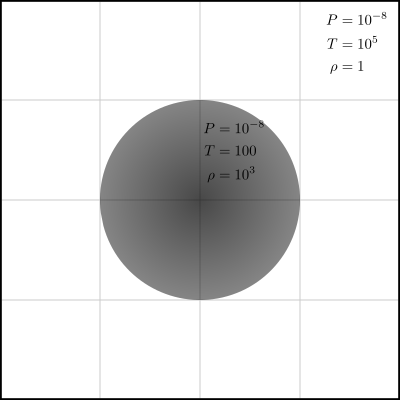
\includegraphics[width=0.7\linewidth]{Images/rect4578.png}
				\caption{Αρχικές συνθήκες ενός στατικού σφαιρικού νέφους ακτίνας \SI{10}{pc}}
				\label{fig:rect4578}
			\end{marginfigure}
		

	
	\subsection{Μονάδες κώδικα}
	Για τις ολοκληρώσεις ο PLUTO χρησιμοποιεί αδιάστατες μεταβλητές για τις ποσότητες πίεσης, πυκνότητας, ταχύτητας, χρόνου και θέσης έτσι ώστε οι αριθμητικές τιμές να εμπίπτουν σε πλαίσια που αποφεύγονται αριθμητικά σφάλματα ($>\num{1e-9},<\num{1e12}$). Στο παρακάτω πίνακα ορίζουμε τις νέες μονάδες, τις οποίες ονομάζουμε και μονάδες κώδικα: 
	
			\begin{table}[H]
				\centering
				\caption{Code Units}
				\label{tab:cd}
				\begin{tabular}{|l|  c |  l|}
					\toprule
					Quantity & Symbol & Code Unit\\ 
					\midrule
					Length & $L_0$ & $\SI{3e19}{\cm} = \SI{10}{pc}$ \\
					Velocity & $V_0$ & $\SI{3e10}{\cm \sec^{-1}}$\\
					Density& $\rho_0$&$\SI{1.67e-24}{g.\cm^3}$\\
					%\multirow{2}{*}{Mass \\ Density} &\multirow{2}{*}{$\rho_0$}  & \multirow{2}{*}{$\SI{1.67e-21}{g. \cm^{-3}}$} \\ \\
					Time & $t_0=\frac{L_0}{V_0}$ & $10^9\si{\sec} =\SI{32}{yrs}$\\
					Pressure & $P_0=\rho_0 V_0^2$ &$\SI{1.5e-3}{dyn.cm^{-2}}$ \\
					Temperature &$T_0=\frac{V_0^2m_p}{k_b}$&$10^{13}\si{\kelvin}$  \\		
					\bottomrule
				\end{tabular}
			\end{table}

	
	\section{Σφαιρικό νέφος μέσα στην ISM}

	Αρχικά θα εκτελέσουμε τη προσομοίωση μας χωρίς καμία "ιδιαίτερη" φυσική διεργασία, δηλαδή θα αφήσουμε ελεύθερο ένα πυκνό σφαιρικό νέφος με τις παραπάνω αρχικές συνθήκες μέσα στο αραιό-θερμό διαγαλαξιακό αέριο.
	
 Όπως παρατηρούμε από το σχήμα~\ref{fig:NoCoolingRHOquad} και καλύτερα από το σχήμα~\ref{fig:nocoolingrhoprofile} μέσα σε 8 εκατομμύρια χρόνια το νέφος είναι στη πράξη σταθερό. 
 
 \begin{marginfigure}
 	\centering
 	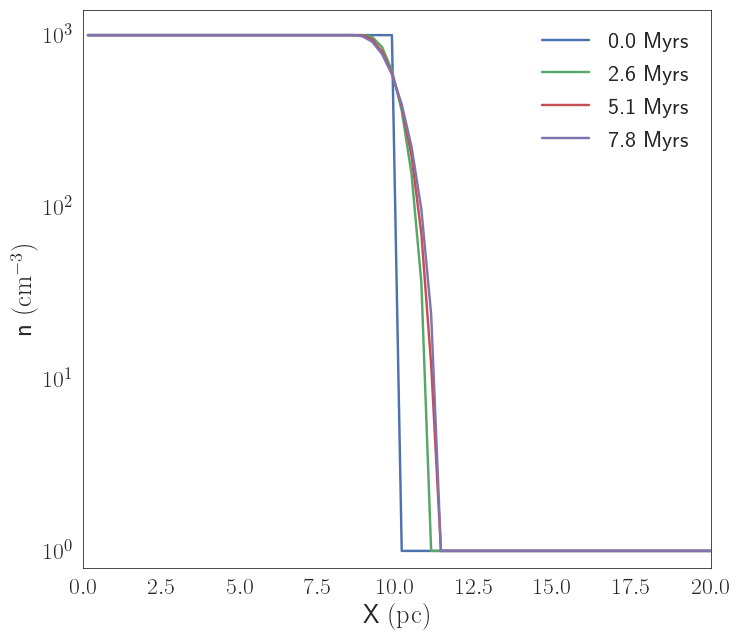
\includegraphics[width=1.0\linewidth]{DataImages/NoCoolingRHOprofile}
 	\caption{Προφίλ της πυκνότητας κατά μήκος της ευθείας $y=0$.}
 	\label{fig:nocoolingrhoprofile}
 \end{marginfigure}	
 
  Η φαινομενική διάχυση που παρατηρούμε είναι αποτέλεσμα αριθμητικών σφαλμάτων στις ταχύτητες (τάξης των \num{1e-18}) καθώς δεν παίρνουμε υπ όψιν μας τη μοριακή διάχυση. Η διάχυση προσθέτει έναν ελλειπτικό όρο στις εξισώσεις με συνέπεια μεγαλύτερη αριθμητική αστάθεια. Καθώς η διάχυση αφορά πολύ μικρές χωρικές κλίμακες τη θεωρούμε αμελητέα.
  Η πίεση παραμένει παντού σταθερή και γι αυτό το σχετικό διάγραμμα παραλείπεται.  
 	
	\begin{figure}[h]
		\centering
		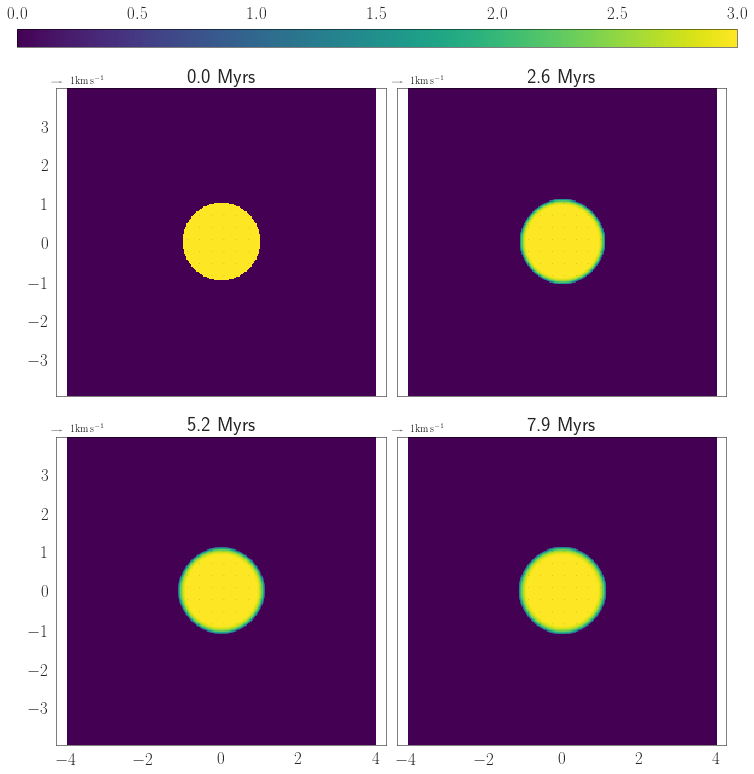
\includegraphics[width=1.0\linewidth]{DataImages/NoCoolingRHOquad}
		\label{fig:NoCoolingRHOquad}
		\caption{Στιγμιότυπα της πυκνότητας ενός σφαιρικού νέφους έως τα 8 εκατομμύρια χρόνια.}
	\end{figure}	
	
	\section{Σφαιρικό νέφος με Radiation Cooling}
	Σκοπός μας είναι να εστιάσουμε στην επιρροή της ψύξης στη δυναμική του αερίου. Ο PLUTO μας δίνει αυτή τη δυνατότητα με τη χρήση διάφορων modules όπου το αέριο ψύχεται καθώς ακτινοβολεί (Radiation Cooling). 

	\subsection{Οπτικό βάθος}
	Το νέφος έχει αριθμητική πυκνότητα $\SI{1000}{cm^{-3}}$ άρα το οπτικό βάθος για ένα φωτόνιο που εκπέμπεται μέσα στο νέφος είναι:
	\begin{equation}
	\tau = nL\sigma _T\simeq \num{6.65e-3}
	\end{equation}
	όπου $\sigma _T = \SI{6.65e-25}{cm^2}$ είναι η ενεργός διατομή Thomson.
	
	Έτσι μπορούμε να συμπεράνουμε οτι είναι οπτικά αδιαφανές, άρα θεωρούμε ότι η ψύξη θα γίνεται ταυτόχρονα σε όλο τον όγκο του νέφους. 
	
	\subsection{Tabulated Cooling}
	Το πρώτο cooling module που θα χρησιμοποιήσουμε ονομάζεται Tabulated Cooling, το οποίο υπολογίζει τον όρο ψύξης $\Lambda (T )$ στην εξίσωση ενέργειας 
	\begin{equation}
		\pdv{t}(\rho e)=-\Lambda^*(n,T)=-n^2 \Lambda(T)
	\end{equation}
	
		\begin{marginfigure}
		%\centering
		\caption{Παράμετρος ψύξης $\Lambda$}
		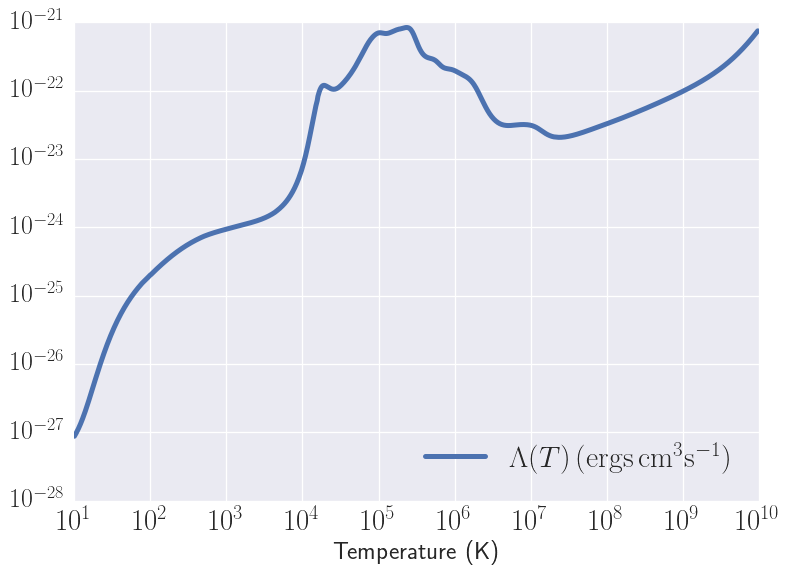
\includegraphics[width=1.0\linewidth]{Images/LambdaT}
		\label{fig:LambdaT}
	\end{marginfigure}
 με αριθμητικές τιμές από έναν εμπειρικό πίνακα καθώς δεν έχουμε αναλυτική μορφή τη συνάρτησης ψύξης. 
 Η μορφή της $\Lambda(T)$ εξαρτάται από τη μεταλλικότητα του αερίου, καθώς οι γραμμές εκπομπής (για θερμοκρασίες \SIrange{1e4}{1e7}{K}) των μετάλλων κυριαρχούν. Για θερμοκρασίες ανώτερες των \SI{1e7}{K} κυριαρχεί η ακτινοβολία bremmstrahlung ενώ για χαμηλότερες των \SI{1e4}{K} η ψύξη προέρχεται από μοριακές εκπομπές (\ce{H2},\ce{CO} κλπ). 
 
 Οι εμπειρικές τιμές της $\Lambda(T)$ που χρησιμοποιήσαμε έχουν παραχθεί από το λογισμικό cloudy με αναλογίες αντίστοιχες της ηλιακής ατμόσφαιρας φαίνονται στο σχήμα~\ref{fig:LambdaT}) σε μονάδες $ \si{ergs.\cm^3 s^{-1}}$ και για  $n=\frac{\rho}{\mu m_u}$.

Η "απλότητα" του συγκεκριμένου module το οποίο δεν συμπεριλαμβάνει τις χημικές διεργασίες, όπως θα δούμε παρακάτω, του προσδίδει αφενός το πλεονέκτημα των χαμηλών υπολογιστικών απαιτήσεων αλλά και την ευκολία στο να κάνουμε μια πρώτη εκτίμηση της χρονικής εξέλιξης των φαινομένων.      
	
	
	\begin{marginfigure}
	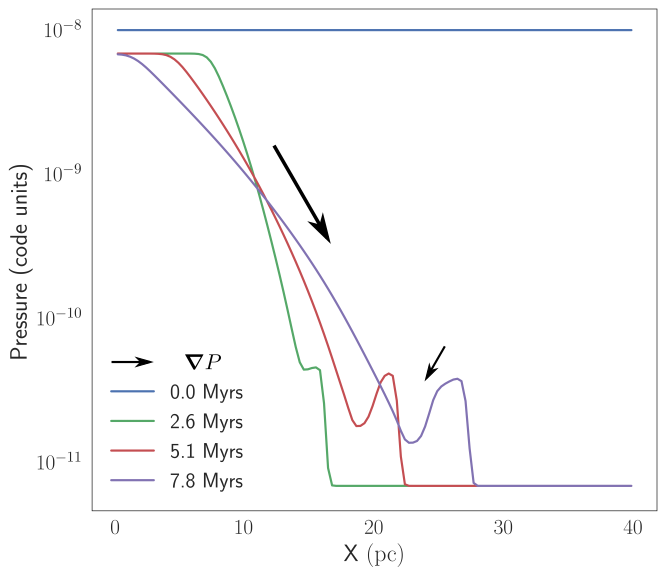
\includegraphics[width=1\linewidth]{DataImages/TabCoolingPRSprofile-gradP}
	\caption{Το προφίλ της πίεσης του αερίου με ενεργοποιημένο το Tabulated Cooling Module κατά μήκος της ευθείας $y=0$ με το χρόνο. Ενδεικτικά (εκτός κλίμακας) δείχνουμε και τη κλίση της πίεσης.}
	\label{fig:tabcoolingprsprofile-gradp}
\end{marginfigure}

	
	
	\subsubsection{Χρονική κλίμακα ψύξης}
	Για μια αρχική θερμοκρασία $T=\SI{100}{K}$ και αριθμητική πυκνότητα $n=10^3\si{cm^{-3}}$ από την εξίσωση της ενέργειας μπορούμε να εκτιμήσουμε τη χρονική κλίμακα ψύξης του νέφους:
%	\marginpar{\centering $k_b=\SI{1.38e-16}{ergs.K^{-1}}$}
	\begin{equation}
		\tau _c =\frac{ \rho e} {n^2 \Lambda (T)}=
		\frac{ \frac{3}{2}k_b T} {n \Lambda (T)} 
		\simeq 10^8\si{s}\simeq \SI{3}{yrs}
	\end{equation}
	Βλέπουμε ότι η χρονική κλίμακα ψύξης είναι τάξης ετών, δηλαδή εξαιρετικά μικρή σε σχέση με τους χρόνους που προσομοιώνουμε (τάξης $10^5\si{yrs}$) και τους χρόνους δυναμικής των νεφών γενικά.
	
	Εδώ πρέπει να σημειωθεί ότι καθώς τα modules που θα χρησιμοποιήσουμε μελετούν μόνο τη ψύξη του αερίου και όχι τη θέρμανση του, για παράδειγμα μέσω κοσμικής ακτινοβολίας, το μεσοαστρικό αέριο 
	
	Αν υπολογίσουμε την αντίστοιχη χρονική κλίμακα και για το εξωτερικό του νέφους βρίσκουμε περίπου \SI{600}{yrs}. 
	
	

	\subsubsection{Δυναμική του νέφους}
	
	Το αέριο στο εσωτερικό του νέφους κρυώνει γρηγορότερα απ' ότι στο εξωτερικό περιβάλλον με συνέπεια η πίεση $P \sim \rho T$ να μικραίνει γρηγορότερα στο εσωτερικό (εφόσον αρχικά είναι ίδια παντού). Αυτή η διαφορά πίεσης δημιουργεί μια  δύναμη η οποία θα έπρεπε να επιταχύνει το αέριο προς το εσωτερικό του. 
	
\begin{marginfigure}
	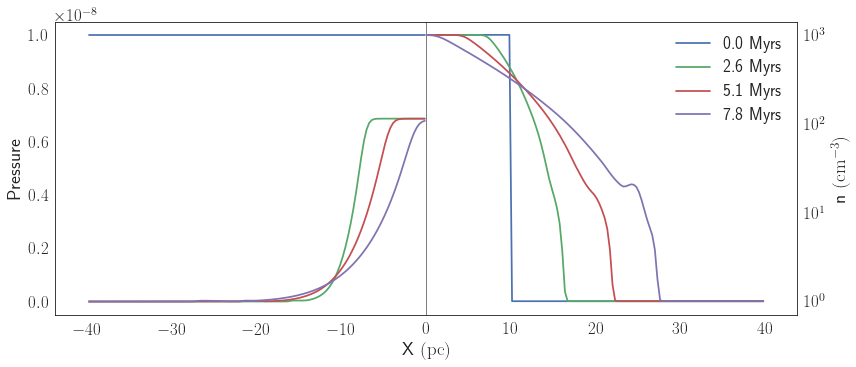
\includegraphics[width=1\linewidth]{DataImages/TabCoolingRHOprofile}
	\caption{Το προφίλ της πυκνότητας του αερίου με ενεργοποιημένο το Tabulated Cooling Module κατά μήκος της ευθείας $y=0$ με το χρόνο.} 
	\label{fig:tabcoolingrhoprofile}
\end{marginfigure}
	
	
\begin{marginfigure}
	\centering
	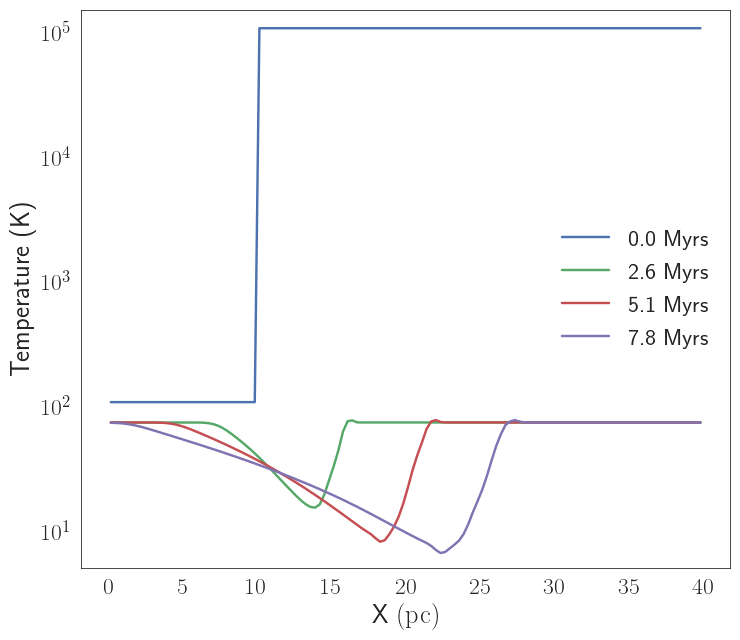
\includegraphics[width=1\linewidth]{DataImages/TabCoolingTMPprofile}
	\caption{Το προφίλ τη θερμοκρασίας με ενεργοποιημένο το Tabulated Cooling Module κατά μήκος της ευθείας $y=0$ με το χρόνο}
	\label{fig:tabcoolingtmpprofile}
\end{marginfigure}
	
	
	\begin{figure}[h]
		\centering
		\caption{Ο χάρτης της πυκνότητας του νέφους στο χρόνο σε λογαριθμική κλίμακα.}
		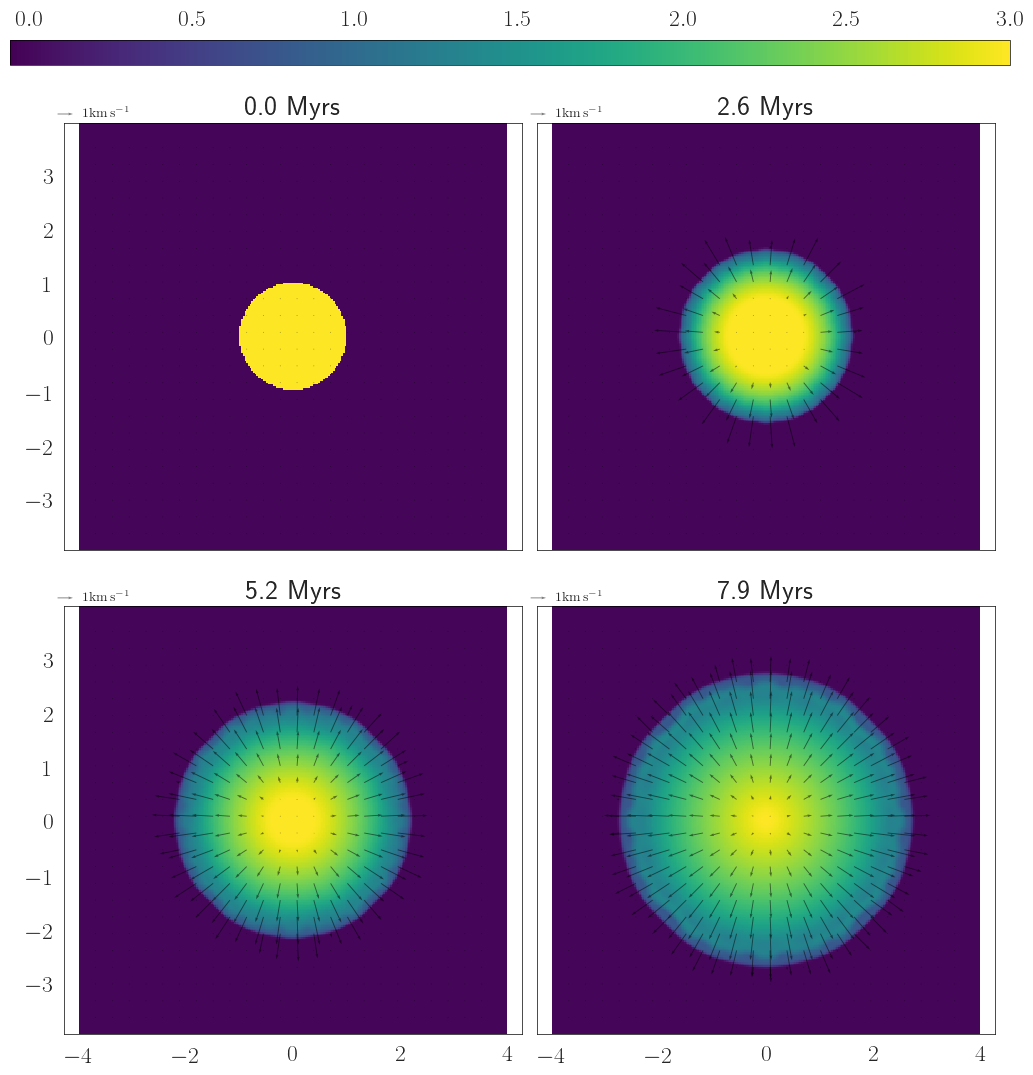
\includegraphics[width=1.0\linewidth]{DataImages/TabCoolingRHOquad}
		\label{fig:TabCoolingRHOquad}
	\end{figure}
		
	
	Από τις προσομοιώσεις όμως, βλέπε σχήματα (\ref{fig:tabcoolingprsprofile-gradp},\ref{fig:tabcoolingprsprofile-gradp}) παρατηρούμε το αντίθετο αποτέλεσμα, δηλαδή μια διαφορά πίεσης με φορά δύναμης προς τα έξω. 

\begin{figure}
	\centering
	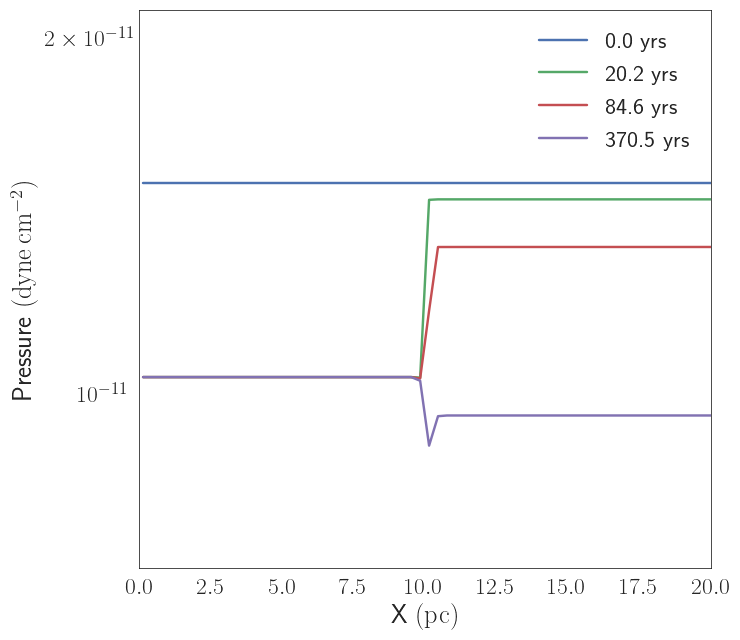
\includegraphics[width=1\linewidth]{DataImages/TabCoolingPRSprofile-micro}
	\caption{}
	\label{fig:tabcoolingprsprofile-micro}
\end{figure}

	
\begin{marginfigure}
	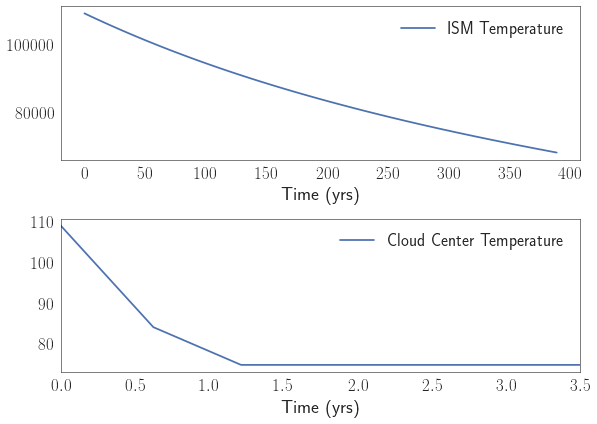
\includegraphics[width=1\linewidth]{DataImages/TabCoolingTMPcenterISM}
	\caption{Η θερμοκρασία στο κέντρο του νέφους συναρτήσει του χρόνου σε ακρίβεια τάξης ετών}
	\label{fig:tabcoolingtmpcenter}
\end{marginfigure}
	
	Για να μελετήσουμε αυτή τη "παράδοξη" συμπεριφορά διαφορά επαναλάβαμε την προσομοίωση σε χρόνους τάξης ετών. Όπως βλέπουμε από το γράφημα~\ref{fig:tabcoolingtmpcenter} η θερμοκρασία στο εσωτερικό όντως μειώνεται αρκετά γρηγορότερα από το εξωτερικό με αποτέλεσμα τη δημιουργία ισοζυγίου δύναμης προς το εσωτερικό.
	
		Καθώς όμως ξεπερνάμε τη χρονική κλίμακα ψύξης του αερίου αυτή ψύξη πρακτικά  σταματάει λόγω του οτι η θερμοκρασία του νέφους άγγιξε κάποια ελάχιστη τιμή, περίπου στους $\SI{70}{K}$. 

 	Το ISM έχοντας πολύ υψηλότερη αρχική θερμοκρασία, μικρότερη πυκνότητα και μεγαλύτερη χρονική κλίμακα ψύξης συνεχίζει να ρίχνει τη πίεση του μέχρι που αυτή ξεπερνάει τη πίεση του νέφους αντιστρέφοντας τη διαδικασία και ξεκινώντας τη διαστολή του νέφους (βλέπε και σχήμα~\ref{fig:tabcoolingprsprofile-micro}).
	

	\subsubsection{Crossing Time}
	\label{par:crossing_time}
%	Ο σκοπός μας είναι να εξετάζουμε βήμα - βήμα τη δυναμική των νεφών. Παρότι εντοπίσαμε το παραπάνω σφάλμα, το οποίο θα προσπαθήσουμε να λύσουμε με την εφαρμογή διαφορετικών modules ψύξης, θα εξετάσουμε ακόμα μια παράμετρο του γενικού μας προβλήματος.
%	
	 Από την εξίσωσης της ορμής:
	\begin{equation}
	\dv{\va V}{t}=-\frac{\grad P}{\rho}
	\end{equation}
	η διαφορά πίεσης που εμφανίζεται λόγο διαφορετικού ρυθμού (και κυρίως τερματισμού της) ψύξης των δύο αερίων δημιουργεί μια δύναμη ακτινικά προς τα έξω η οποία διαστέλλει το νέφους. Ουσιαστικά η διαστολή αυτή είναι η μετάδοση δύο κυμάτων. Ενός κύματος συμπύκνωσης προς το εξωτερικό το οποίο συνοδεύεται από ένα κύμα αραίωσης στο εσωτερικό. Δηλαδή εν τέλει έχουμε μια φαινομενική "κατάρρευση" του νέφους, αφού η φαινομενική ακτίνα του (δηλαδή η ακτίνα εκείνη που διατηρεί την αρχική πυκνότητα) μικραίνει.
	 
	Η ταχύτητα διάδοσης αυτής της "κατάρρευσης" δηλαδή η ταχύτητα διάδοσης των δύο κυμάτων είναι η ταχύτητα του ήχου στο εκάστοτε μέσο. Η τοπική ταχύτητα του ήχου είναι:
	\begin{equation}
	c_s=\sqrt{\gamma \frac{P}{\rho}}
	\end{equation}
	όπου $\gamma = 5/3$
	
	
	Από τις αρχικές συνθήκες (παράγραφος~\ref{par:InitialConditions}) οι τοπικές ταχύτητες του ήχου για το εσωτερικό και το εξωτερικό είναι:
	\begin{align}
	c_s &=\SI{1.2}{km.s^{-1}} \qq{(MC)} \\
	c_s &=\SI{38.7}{km.s^{-1}} \qq{(ISM)}
	\end{align}
	
	Καθώς η πίεση πέφτει, η ταχύτητα του ήχου στο νέφος μειώνεται κατά ένα παράγοντα $\sim 0.75^{1/2}=0.8$ δηλαδή περίπου $1\si{.km.s^{-1}}$.
	
%	\begin{marginfigure}
%		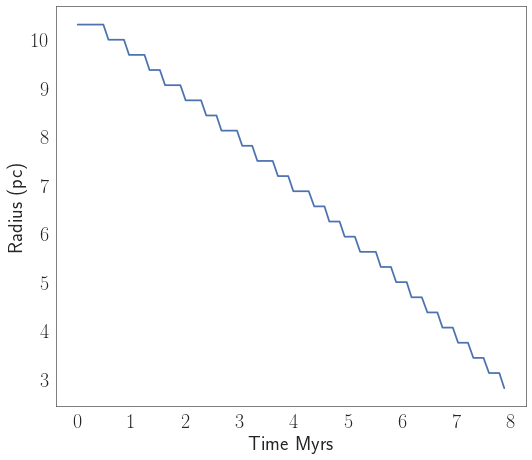
\includegraphics[width=1\linewidth]{DataImages/TabCoolingRadius}
%		\caption{Εκτίμηση της ακτίνας του νέφους συναρτήσει του χρόνου. Υπολογίστηκε με βάση τη παράγωγο του προφίλ της πυκνότητας κατά μήκος της ευθείας $y=0$}
%		\label{fig:tabcoolingradius}
%	\end{marginfigure}
%	
	Άρα τώρα μπορούμε να εκτιμήσουμε τη χρονική κλίμακα της "κατάρρευσης" με βάση την ακτίνα του νέφους:
	\begin{equation}
	\tau_R=\frac{R}{c_s} \simeq \SI{7.5}{\mega yrs}
	\end{equation}
	το οποίο φαίνεται να συμφωνεί με τη παρατήρηση, βλέπε σχήμα~\ref{fig:tabcoolingradius}.
	
	\subsubsection{Πρώτα Συμπεράσματα}
	Με τη χρήση του Tabulated Cooling Module του PLUTO δείξαμε ότι η προσπάθεια προσομοίωσης της δυναμική ενός σχετικά κρύου αερίου ότι οδηγεί σε μια σχεδόν κατώτατη θερμοκρασία η οποία προκύπτει από τη απότομη αύξηση της κλίσης της καμπύλης ψύξης.
	
	Παρότι δίνει ικανοποιητικά αποτελέσματα η σταθερότητα της είναι μη ρεαλιστική (καθώς η μεταλλικότητα και η αναλογία ιόντων μπορεί να αλλάζει ανά περιοχή και ανά χρονο) κάτι που κρίνουμε οτί προς το παρόν δεν μας καλύπτει.
	
%	\todo{Καλλιοπη: Ακόμα δεν μπορω να καταλάβω γιατι τελικά σταματαει τόσοοο αποτομα η θερμοκρασια. Το αποτελεσμα αυτο συμφωνει και με το H2COOL όπου εκει βεβαια περνει εκατομμυρια χρονια για να φτασει. Μήπως τελικά οι δυο τάξης μεγέθους διαφορα στην cooling function αρκουν για να επιβραδύνουν αρκετα τη ψύξη σταθεροποιώντας τη θερμοκρασία στους 70~90 K. }
%	
%	Παρότι θα μπορούσαμε να επεκτείνουμε μέσω τεχνικών παρεμβολής τον πίνακα  $\Lambda (T)$ κρίναμε ότι κάτι τέτοιο απλά θα προσφέρει μια νέα χαμηλότερη θερμοκρασία και άρα μια επανάληψη των ίδιων περίπου αποτελεσμάτων με μια σχετική χρονική καθυστέρηση. 
%	
%	Άρα χρειαζόμαστε μια νέα προσέγγιση του όρου ψύξης στις χαμηλές θερμοκρασίες ώστε να αποκομίσουμε μια ρεαλιστικότερη απεικόνιση της εξέλιξης ενός κρύου αερίου μέσα στο διαγαλαξιακό μέσο.  
%	
%	Με βάση ένα εσφαλμένο μοντέλο έχουμε ενδείξεις για το πόσο σημαντικό ρόλο παίζει, σε νέφη τεραστίων διαστάσεων η ψύξη στις πολύ μικρές θερμοκρασίες. 
%	
	\subsection{SNEq Cooling}
	Με βάση τα παραπάνω θα εξετάσουμε το δεύτερο module ψύξης μέσω ακτινοβολίας οπτικά αραιού μέσου του PLUTO, το οποίο ονομάζεται \textbf{Simplified Non-Equilibrium Cooling (SNEq)}. 
	
	Για να χρησιμοποιήσουμε το SNEq θα πρέπει να ορίσουμε σαν μια ακόμη μεταβλητή την
	αναλογία ουδετέρου Υδρογόνου σε σχέση με το Πλάσμα.
	Σε κάθε βήμα της προσομοίωσης ο κώδικας ολοκληρώνει μαζί με τις υδροδυναμικές εξισώσεις και την χρονική μεταβολή του $x_{\ce{HI}}$ μέσω της εξίσωσης:
	\begin{equation}
	\pdv{x_{\ce{HI}}}{t}=n_e \left( -(c_r+c_i)f_n+c_r\right) 
	\end{equation}
	μαζί με την εξίσωση της ενέργειας ή οποία γίνεται:
	\begin{equation}
	\pdv{t}(\rho e)=-\Lambda=-n_e n_{\ce{H}} \left( \sum\limits_{k=1}^{16}j_k +w_{i/r} \right) 
	\end{equation}
	
	όπου η άθροιση στα $k$ υπολογίζει 16 διαφορετικές γραμμές εκπομπής 
	(Ly α, H α, HeI (584+623), CI (9850 + 9823), CII (156μ), CII (2325Å), NI (5200 Å),
	NII (6584 + 6548 Å), OI (63μ), OI (6300 + 6363 Å), OII (3727), MgII (2800), SiII (35μ), SII (6717 + 6727),FeII (25μ), FeII (1.6μ))
	
	Ο συντελεστής $j_k$ έχει μονάδες $\si{erg/sec . cm^3}$ και υπολογίζεται από τη σχέση:
	\begin{equation}
	j_k=\frac{\hbar^2 \sqrt{2\pi}}{\sqrt{k_B m_e}m_e}f_k q_{12}\frac{h \nu _k}{1+n_e (q_{21}/A_{21})}
	\end{equation}
	με $k$ τον δείκτη της εκάστοτε μετάπτωσης και $f_k=n_k/n_{\ce{H}}$ το ποσοστό του εκάστοτε στοιχείου.
	\begin{align}
	q_{12}=\frac{\num{8.6e-6}}{\sqrt{T}}\frac{\Omega _{12}}{g_1}e^{-\frac{h\nu _k}{k_B T}} 
	&&
	q_{21}=\frac{\num{8.6e-6}}{\sqrt{T}}\frac{\Omega _{21}}{g_2}
	\end{align} 
	με $\Omega _{12} = \Omega _{21}$ η ισχύς της σύγκρουσης με τιμές οι οποίες είναι καταγεγραμμένες σε πίνακα.
	Το $w_{i/r}$ αντιπροσωπεύει τη θερμική ενέργεια που χάνεται από τον ιονισμό και την επανασύνδεση:
	\begin{equation}
	w_{i/r} = c_i\times \num{13.6}\times \num{1.6e-12} f_n +c_r \times \num{0.67}\times \num{1.6e-12} (1-f_n) \frac{T}{11590}
	\end{equation}
	όπου $c_r$ και $c_i$ είναι οι ρυθμοί ιονισμού και επανασύστασης του Υδρογόνου:
	\begin{align}
	c_r=\frac{\num{2.6e-11}}{\sqrt{T}} 
	&& 
	c_i=\frac{\num{1.08e-8}\sqrt{T}}{\num{13.6}^2} e^{-\frac{\num{157890}}{\sqrt{T}}}
	\end{align}
	
	
	\subsubsection{Προσομοίωση με SNEq Cooling}
	
			\begin{figure}
				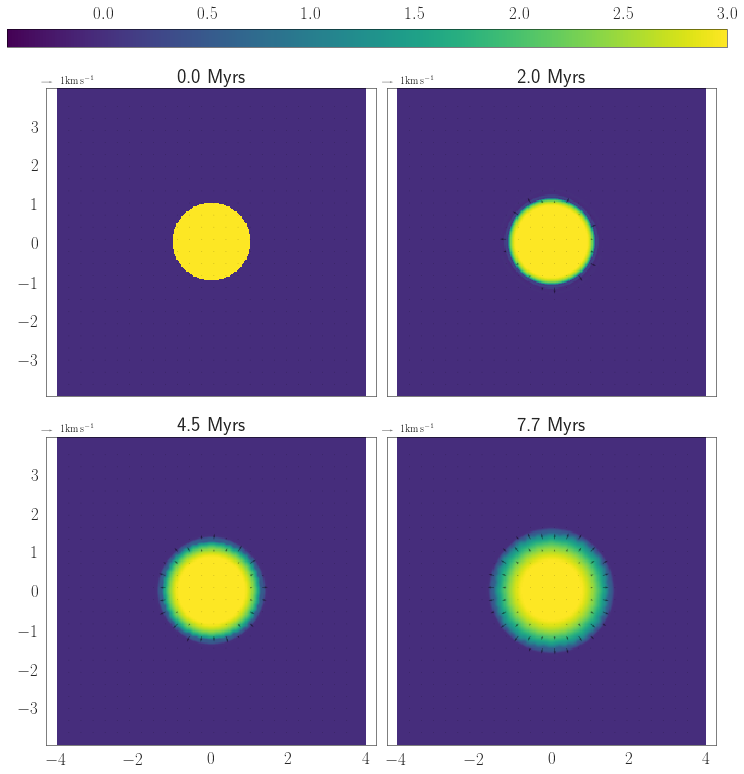
\includegraphics[width=1\linewidth]{DataImages/SNCoolingRHOquad}
				\caption{Ο χάρτης της πυκνότητας του νέφους για τη προσομοίωση του SNEq Cooling στο χρόνο (σε λογαριθμική κλίμακα).}
				\label{fig:sncoolingrhoquad}
			\end{figure}
		
\begin{marginfigure}
	\centering
	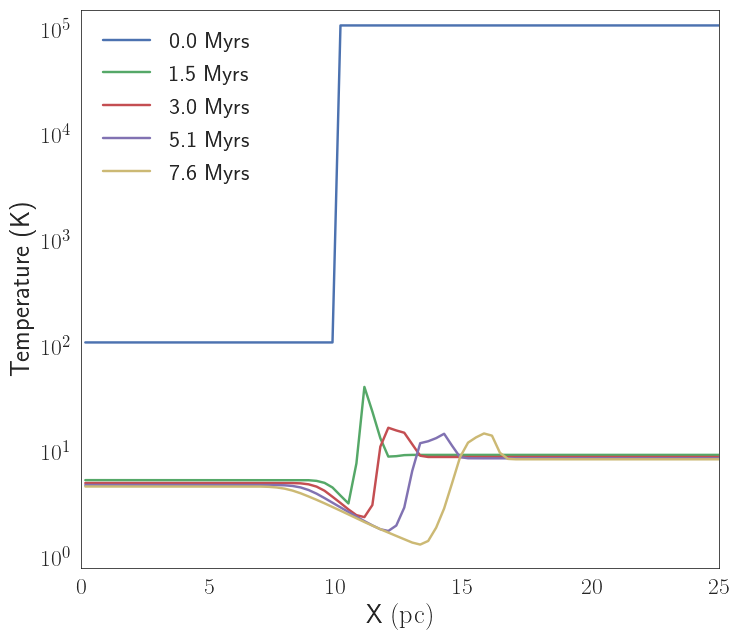
\includegraphics[width=1\linewidth]{DataImages/SNCoolingTMPprofile}
	\caption{}
	\label{fig:sncoolingtmpprofile}
\end{marginfigure}

\begin{marginfigure}
	\centering
	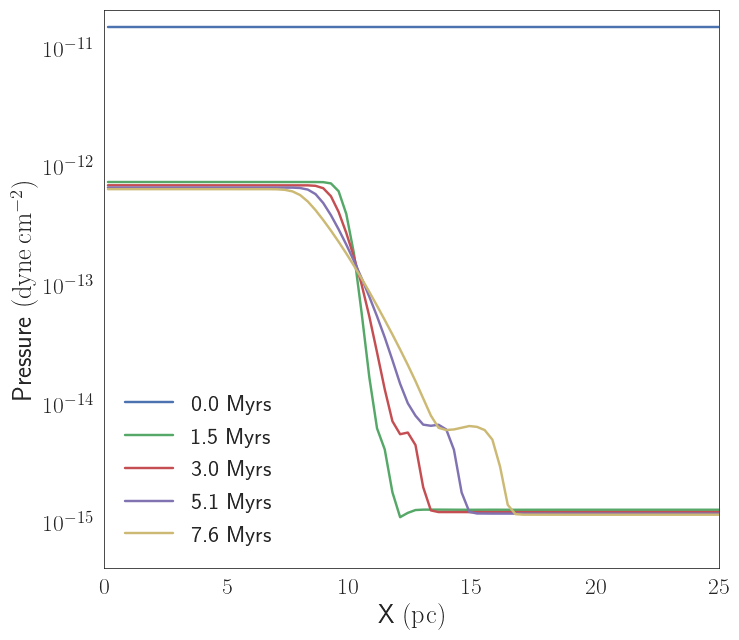
\includegraphics[width=1\linewidth]{DataImages/SNCoolingPRSprofile}
	\caption{}
	\label{fig:sncoolingprsprofile}
\end{marginfigure}
	
	Δεχόμενοι σαν βάση τη προηγούμενη προσπάθεια μας και τις ίδιες αρχικές συνθήκες για να χρησιμοποιήσουμε το SNEq Cooling Module θα πρέπει να ορίσουμε το ποσοστό ουδετέρου Υδρογόνου $x_{\ce{HI}}$.
	
\begin{figure}[h]
	\centering
	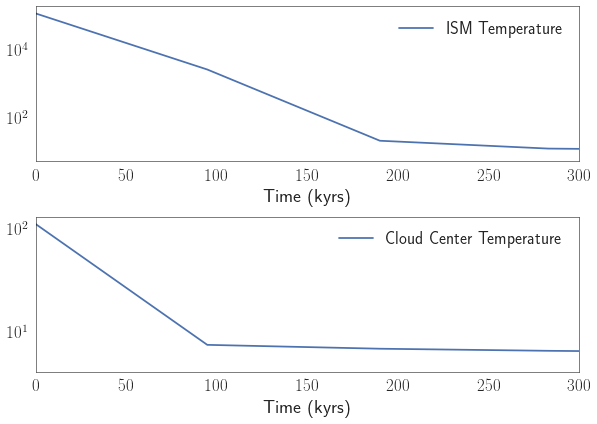
\includegraphics[width=1\linewidth]{DataImages/SNCoolingTMPcenterISM}
	\caption{Θερμοκρασία (αριστερή κλίμακα) και ποσοστό ουδετέρου υδρογόνου (διακεκομμένη καμπύλη, δεξιά κλίμακα) για το μεσοαστρικό αέριο (επάνω σχήμα) και εσωτερικό του νέφους (κάτω σχήμα)}
	\label{fig:sncoolingtmpcenterism} 
\end{figure}
	
	Για να ελέγξουμε την ευστάθεια των χημικών διεργασιών θεωρήσαμε σαν αρχική συνθήκη το ποσοστό του ουδετέρου υδρογόνου να είναι στο εσωτερικό του νέφους $x_{\ce{HI}}=0.1$ οπότε θα περιμέναμε λόγω της χαμηλής θερμοκρασίας και υψηλής πυκνότητας το ποσοστό αυτό να αυξηθεί. Στο εξωτερικό του νέφους, με το ίδιο σκεπτικό, χρησιμοποιούμε τη τιμή $x_{\ce{HI}}=0.9$ οπότε αντίστοιχα περιμένουμε λόγω της υψηλής θερμοκρασίας και της χαμηλής πυκνότητας σχεδόν ολόκληρο το υδρογόνου να είναι σε ατομική μορφή. 
	
	Όπως παρατηρούμε και από το σχήμα \ref{fig:sncoolingtmpcenterism} η συμπεριφορά είναι όντως η αναμενόμενη εκτός από το μεσοαστρικό χώρο ο οποίος κρυώνει σε πολύ μικρό χρονικό διάστημα αναγκάζοντας το ποσοστό ουδετέρου υδρογόνου να μειώνεται έως ότου η χαμηλή θερμοκρασία να το επαναφέρει στο 100\%. 
	
	Αντίστοιχα, για το πλήρη έλεγχο, εκτελέσαμε τη προσομοίωση με τα αντίστροφα ποσοστά με ταυτόσημα αποτελέσματα οπότε και παραλείψαμε τα σχετικά διαγράμματα.


Η θερμοκρασία του νέφους φτάνει σε τιμές κάτω των $\SI{10}{K}$, κάτι το οποίο έρχεται σε συμφωνία με τα  παρατηρησιακά δεδομένα από τα μοριακά νέφη. Όπως είδαμε και προηγουμένως η θερμοκρασία του μεσοαστρικού χώρου μειώνεται αρκετά γρήγορα κοντά στους \SI{10}{K}.


Λόγω της σχεδόν ισοδύναμης ψύξης του νέφους με το μεσοαστρικό περιβάλλον η διαφορά πίεσης είναι μικρότερη όπως και η ταχύτητα του ήχου στο εσωτερικό του νέφους με αποτέλεσμα η φαινομενική κατάρρευση της κεντρικής περιοχής να είναι πολύ πιο αργή σε σχέση με το Tabulated Cooling. Στο σχήμα \ref{fig:tabsnsoundspeed} παρουσιάζουμε τις διαφορές στη ταχύτητα του ήχου μεταξύ του tabulated Cooling και του SNEq Cooling.

\begin{marginfigure}
	\centering
	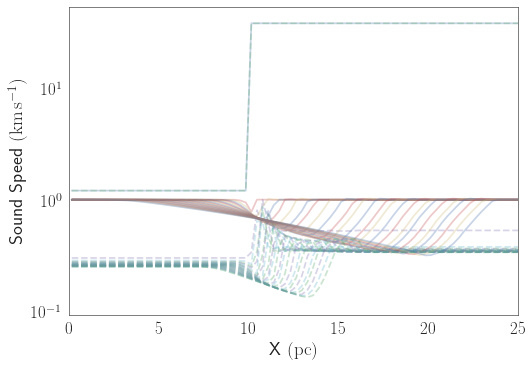
\includegraphics[width=1\linewidth]{DataImages/TabSNSoundSpeed}
	\caption{}
	\label{fig:tabsnsoundspeed}
\end{marginfigure}

Συμπερασματικά παρότι η ψύξη στο εσωτερικό του νέφους αποδίδει πιο ρεαλιστικά αποτελέσματα σε σχέση με τις παρατηρήσεις η καμπύλη ψύξης φαίνεται να μη συμφωνεί καθόλου με τη παρατηρούμενη καμπύλη ψύξης. Κρίνουμε ότι το module SNEq δεν κρίνεται αξιόπιστο για τις ανάγκες μας. 
\begin{figure}
	\centering
	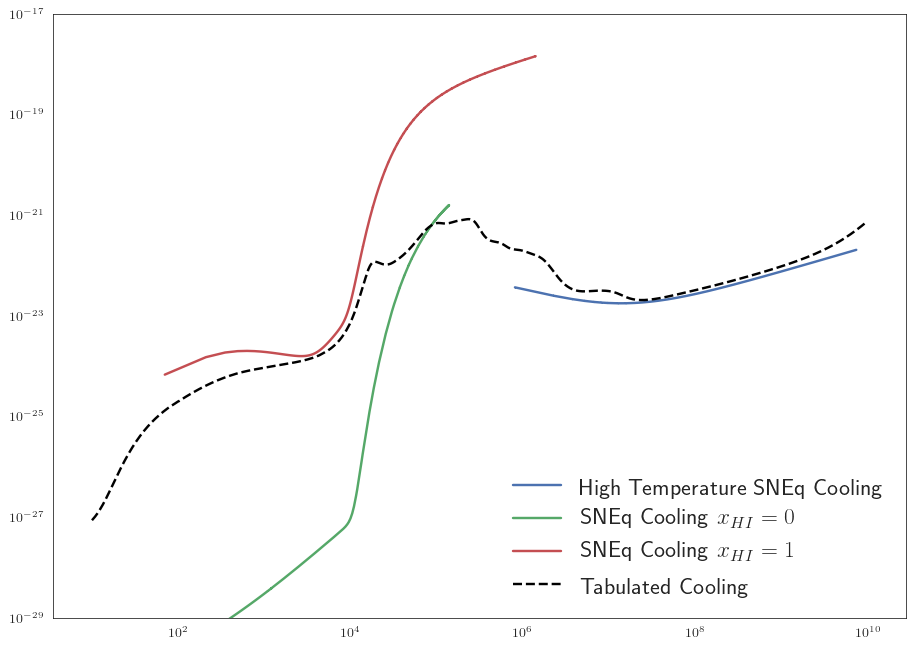
\includegraphics[width=1\linewidth]{DataImages/SNEQcooling-function}
	\caption{}
	\label{fig:sneqcooling-function}
\end{figure}



%	\begin{marginfigure}
%		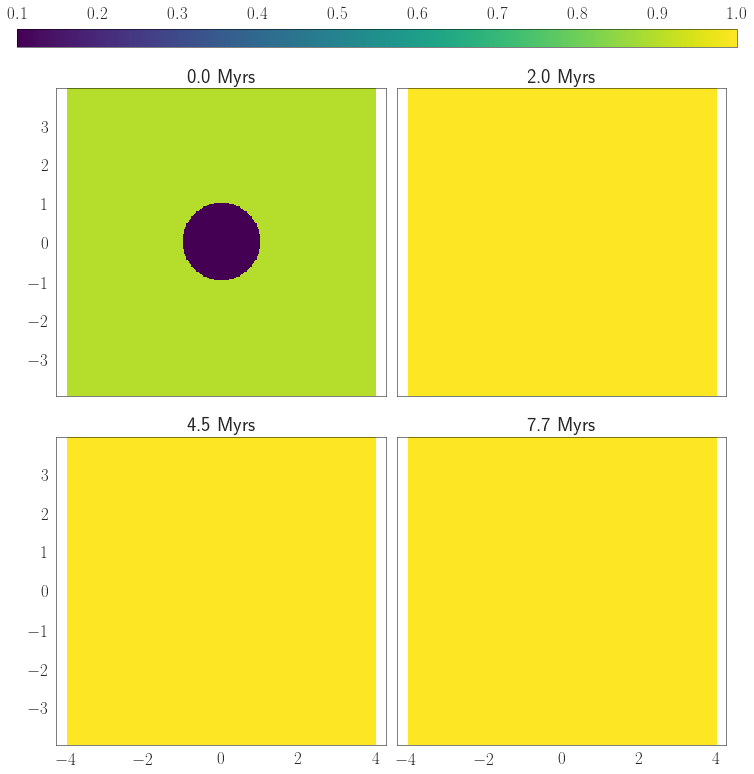
\includegraphics[width=1\linewidth]{DataImages/SNCoolingXHIquad}
%		\caption{Χρονική εξέλιξη του ποσοστού ουδετέρου Υδρογόνου}
%		\label{fig:sncoolingxhiquad}
%	\end{marginfigure}
%	

%\begin{figure}[h]
%	\begin{adjustwidth}{-0cm}{-5cm}	
%	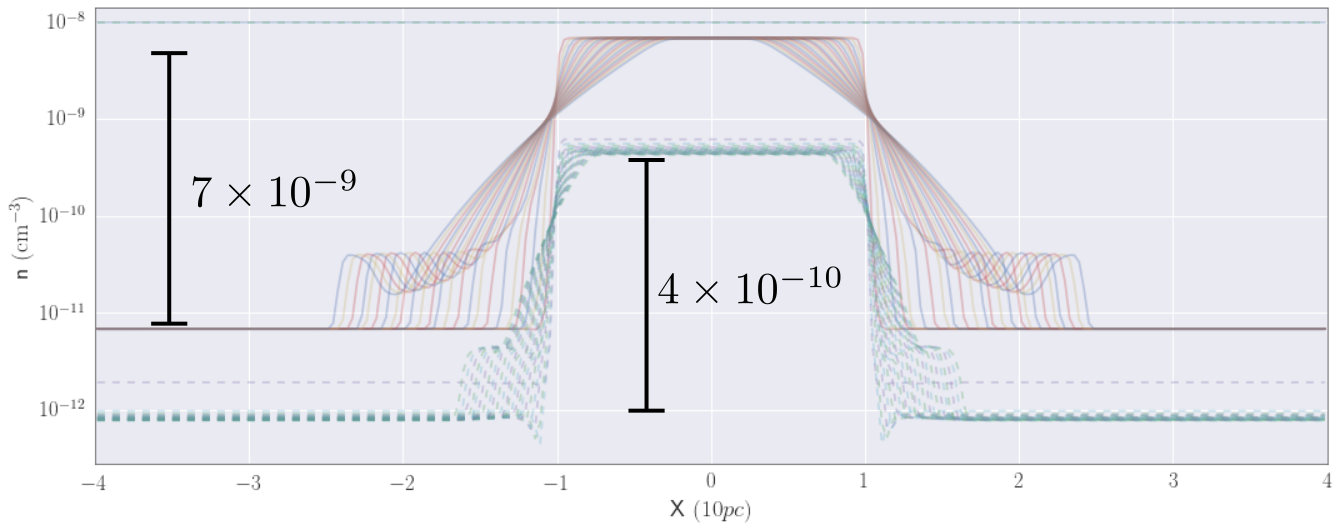
\includegraphics[width=1\linewidth]{DataImages/diffTabCoolSNCoolPRSprofile-edit}
%\caption{Το προφίλ της πίεσης του αερίου με ενεργοποιημένο το SNEq Cooling Module (διακεκομένη γραμμή) σε σύγκριση με αυτή του Tabulated Cooling κατά μήκος της ευθείας $y=0$ με το χρόνο.}
%\label{fig:difftabcoolsncoolprsprofile-edit}
%\end{adjustwidth}
%\end{figure}


\newpage
	\subsection{H2 Cooling}
%	Η ψύξη μέσω του SNEq είχε εμφανώς καλύτερα, δηλαδή πιο ρεαλιστικά αποτελέσματα αλλά διατηρεί ένα μεγάλο πρόβλημα που έχουμε για τις χαμηλές θερμοκρασίες. Οι μαγνητουδροδυναμικοί αριθμητικοί κώδικες αντιλαμβάνονται το ρευστό σαν ιονισμένο πλάσμα. Παρότι σε μεγάλες θερμοκρασίες η προσέγγιση αυτή είναι καλή σε χαμηλές θερμοκρασίες εμφανίζονται ουδέτερα άτομα και μόρια.
	
	Παρότι σε υψηλές θερμοκρασίες η προσέγγιση του αερίου σαν ιονισμένο πλάσμα είναι ικανοποιητική
	σε χαμηλές θερμοκρασίες όπου κυριαρχούν οι μοριακές εκπομπές είναι ανεπαρκής έως και λανθασμένη. Οι περισσότεροι μαγνητοϋδροδυναμικοί αριθμητικοί κώδικες όπως και ο PLUTO επιλύουν τις εξισώσεις μέ τη προσέγγιση του ενός ρευστού το οποίο σημαίνει ότι δυναμικά δεν μπορούμε να αποφύγουμε το μη υπολογισμό φαινομένων της αλληλεπίδρασης των πολλαπλών στοιχείων, μορίων και σκόνης (ειδικότερα αν βάλουμε στο παιχνίδι και μαγνητικά πεδία). 
	
	Tα Cooling modules SNEq και H2Cool δραστηριοποιούνται παράλληλα με την ολοκλήρωση των κινητικών εξισώσεων υπολογίζοντας την εξέλιξη της χημικής σύστασης του αερίου μέσω χημικών δικτύων και με βάση τη πυκνότητα και τη θερμοκρασία.  
	
%	Το SNEq module μέσω του χειρισμού του ποσοστού $x_{H_I}$ έκανε ένα βήμα προς αυτή τη κατεύθυνση αλλά για ένα μοριακό νέφος με μεγάλες ποσότητες σε \ce{H_2}, πληθώρα άλλων μορίων (\ce{He}, \ce{CO} κλπ) μαζί με σκόνη προφανώς η προσέγγιση αυτή δεν είναι αρκετή.
%	
%	Έτσι δοκιμάσαμε και το επόμενο Cooling Module που διαθέτει ο PLUTO το οποίο ονομάζεται \textbf{Molecular Hydrogen Non-Equilibrium Cooling (H2 COOL)}.
	
	Το H2COOL εισάγει με τη σειρά του 2 ακόμα μεταβλητές. Έτσι, εκτός του ποσοστού ουδετέρου υδρογόνου, έχουμε το ποσοστό ιονισμένου υδρογόνου $x_{\ce{HII}}$ και το ποσοστό μοριακού Υδρογόνου $x_{\ce{H2}}$.
	\begin{align}
	x_{\ce{HI}} =\frac{n_{\ce{HI}}}{n_{\ce{H}}} && x_{\ce{HI}} =\frac{n_{\ce{HII}}}{n_{\ce{H}}} && x_{\ce{H2}} =\frac{n_{\ce{H2}}}{n_{\ce{H}}} 
	\end{align}
	όπου η συνολική αριθμητική πυκνότητα του Υδρογόνου $n_H=n_{H_I}+n_{H_{II}}+2n_{H_2}$.
	
	Η χημική εξέλιξη του μοριακού, ατομικού και ιονισμένου υδρογόνου ακολουθεί τις αντιδράσεις:
	\begin{align}
	&\ce{H + e^- -> H^+ + 2e^-} && k_1 = \num{5.84e-11} \sqrt{T} e^{\num{-157809}/T} \\
	&\ce{H^+ + e^- -> H + h\nu} && k_2 = \num{2.6e-11} \sqrt{T}\\
	&\ce{H_2 + e^- -> 2H + e^-} && k_3 = \num{4.4e-10}T^{0.35} e^{\num{-102000}/T}\\
	&\ce{H_2 + H -> 3H} && k_4=\num{1.067e-10}T_{eV}^{2.012} e^{\frac{\num{-4.463}}{T_{eV}}(1+\num{0.2472}T_{eV})^{3.512}}\\
	&\ce{H_2 + H_2 -> H_2 + 2H} && k_5=\num{1.0e-8}e^{-\num{84100}/T} \\
	&\ce{H + H ->[\mathtt{dust}] H_2} && k_6=\num{3.0e-17}\sqrt{T_2} (1+0.4\sqrt{T_2}+0.2 T_2 +0.08 (T_2)^2)
	\end{align}
	όπου $T$ η θερμοκρασία σε Κέλβιν, $T_{eV}$ η θερμοκρασία σε ηλεκτρονιοβόλτ, $T_2=\frac{T}{100}$ και $k_i$ ο ρυθμός εξέλιξης της κάθε αντίδρασης σε $\si{cm^3 s^{-1}}$.
	
	Η εξέλιξη των αριθμητικών πυκνοτήτων υπολογίζεται από την εξίσωση:
	\begin{equation}
	S_i=\dv{n_i}{t}=\sum\limits_{j,k}k_{j,k}n_j n_k - n_i \sum_{j}k_{i,j}n_j
	\end{equation}
	όπου $k_{j,k}$ είναι ο ρυθμός παραγωγής του $i$ στοιχείου από τα υπόλοιπα στοιχεία $j$ και $k$, και $k_{i,j}$ ο ρυθμός καταστροφής του $i$ στοιχείου από όλα τα $j$ στοιχεία.
	
	Ο κώδικας ολοκληρώνει τα ποσοστά των 3 ειδών υδρογόνου μέσω της επίλυσης της παραπάνω εξίσωσης μαζί με την εξίσωση μεταφοράς:
	\begin{equation}
	\pdv{X_i}{t}=-\va{u}\cdot \grad{X_i}+S_i
	\end{equation}
	όπου ο όρος μεταφοράς $-\va{u}\cdot \grad{X_i}$ ολοκληρώνεται μαζί με τις υδροδυναμικές εξισώσεις μάζας, ορμής (hydro step) ενώ ο όρος $S_i$ ολοκληρώνεται κατά το βήμα της ψύξης (cooling step).
	
	Οι ενεργειακές απώλειες λόγω ψύξης τελικά υπολογίζονται, εκτός από τις παραπάνω αντιδράσεις, από τις απώλειες ιονισμού λόγω κρούσης $\Lambda _{\mathtt{CI}}$ και επανασύνδεσης λόγω ακτινοβολίας $\Lambda _{\mathtt{RR}}$, απώλειες λόγω περιστροφής και ταλάντωσης (rotational-vibrational cooling) $\Lambda _{\mathtt{rotvib}}$ και διάσπασης (dissosiation) $\Lambda _{\mathtt{diss}}$ των μορίων \ce{H_2}, και της διαδικασίας αλληλεπίδρασης σκόνης-αερίου (gas-grain process) $\Lambda _{\mathtt{grain}}$.
	\begin{equation}
	\Lambda = \Lambda _{\mathtt{CI}} + \Lambda _{\mathtt{RR}} +\Lambda _{\mathtt{rotvib}} + \Lambda _{\mathtt{diss}} + \Lambda _{\mathtt{grain}}
	\end{equation}
	
	\todo[inline]{Depending on the requirement, the user can add more components to the cooling function, for e.g., cooling due to fixed fractions of standard molecules like CO, OH, H 2 O etc or contributions from collisional excitation of lines as indicated in the SNEq module.}
%
%	\begin{marginfigure}
%	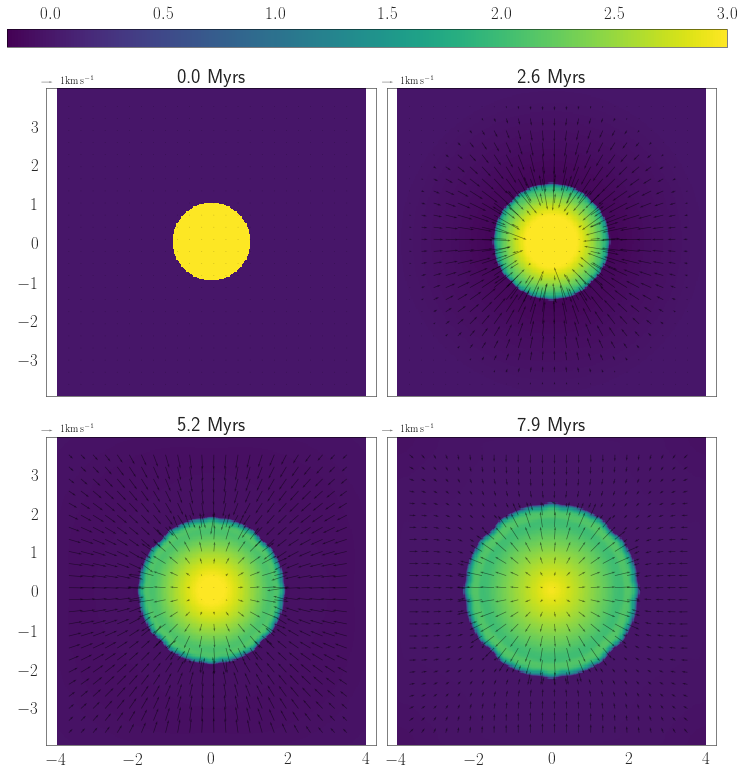
\includegraphics[width=1.\linewidth]{DataImages/H2CoolingRHOquad}
%	\caption{Η πυκνότητα του αερίου σε διάφορες χρονικές στιγμές}
%	\label{fig:h2coolingrhoquad}
%\end{marginfigure}	

	\subsubsection{Προσομοίωση με H2COOL}
		\marginpar{
		\begin{table}[H]
			\caption{}Αρχικές συνθήκες για τα ποσοστά των \newline
				διαφορετικών μορφών Υδρογόνου \newline
			\label{tab:h2sc}
			\begin{tabular}{|l|  c |  c| c|}
				\toprule
				Περιοχή & $x_{\ce{H_Ι}}$ & $x_{\ce{H_{ΙΙ}}}$ & $x_{\ce{H_2}}$ \\ 
				\midrule
				Μοριακό Nέφος & $0.1$ & $0$ & $0.9$ \\
				Μεσογαλαξιακό μέσο  & $0.9$ & $0.1$ & $0$ \\
				\bottomrule
			\end{tabular}
		\end{table}
	}

	Ακολουθώντας την ίδια πορεία με προηγουμένως ορίζουμε στις αρχικές συνθήκες τα ποσοστά μοριακού, ουδετέρου και ιονισμένου υδρογόνου όπως φαίνονται στο πίνακα~\ref{tab:h2sc}.
	
	\begin{marginfigure}
		\centering
		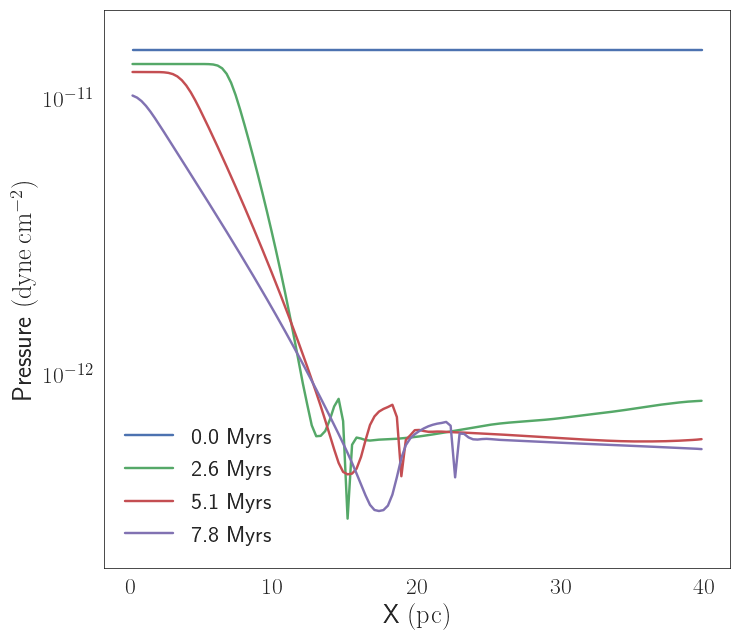
\includegraphics[width=1\linewidth]{DataImages/H2CoolingPRSprofile}
		\caption{}
		\label{fig:h2coolingprsprofile}
	\end{marginfigure}
	
	\begin{marginfigure}
		\centering
		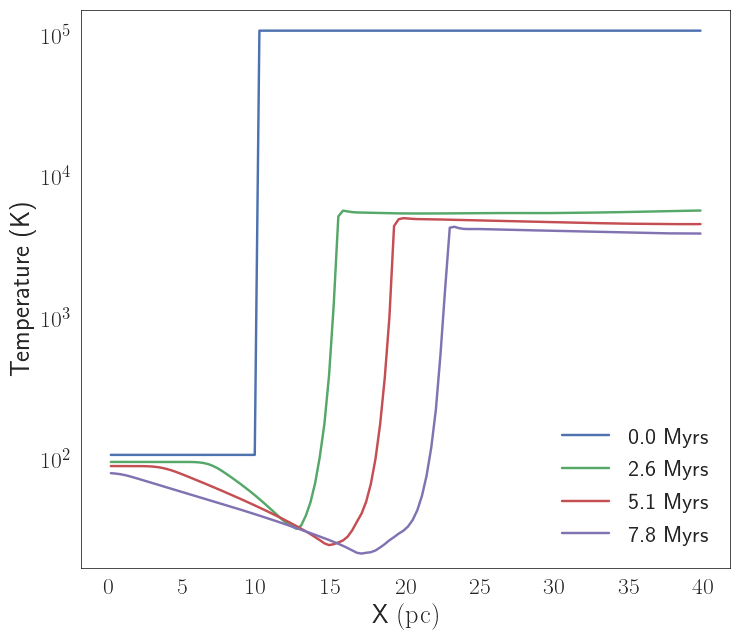
\includegraphics[width=1\linewidth]{DataImages/H2CoolingTMPprofile}
		\caption{}
		\label{fig:h2coolingtmpprofile}
	\end{marginfigure}
	
	
\begin{figure}[h]
	\centering
	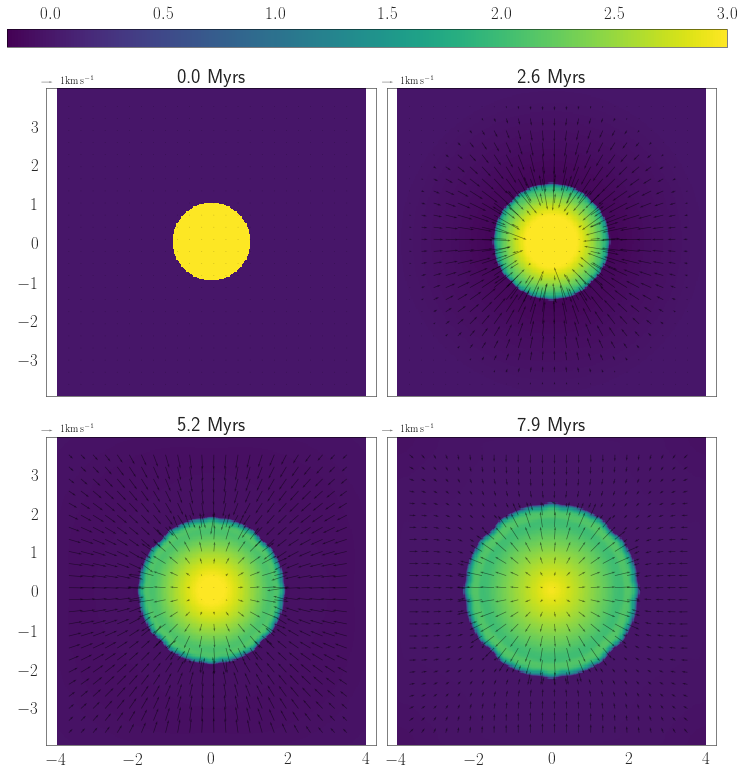
\includegraphics[width=1\linewidth]{DataImages/H2CoolingRHOquad}
	\caption{}
	\label{fig:h2coolingrhoquad}
\end{figure}


	Το πρώτο που παρατηρούμε είναι ότι το νέφος διαστέλλεται σε χρονική κλίμακα τάξης του crossing time. Ο λόγος είναι γιατί η διαφορά πιέσεων είναι πολύ μεγαλύτερη καθώς το κεντρικό τμήμα του νέφους διατηρεί τη πίεση στα ίδια επίπεδα με την αρχική πίεση $10^{-8}$. Για να αλλάξει η πυκνότητα στο εσωτερικό του νέφους χρειάζεται ένας αρκετά μεγάλος χρόνος, άρα η σχετική στασιμότητα της πίεσης σημαίνει και στασιμότητα της θερμοκρασίας. Όντως όπως βλέπουμε και στο σχήμα~\ref{fig:h2coolingtmpprofile} η θερμοκρασία του νέφους μειώνεται πάρα πολύ αργά (τάξης εκατομμυρίων ετών ενώ η αντίστοιχη σε μέγεθος μείωση της θερμοκρασίας για το Tabulated Cooling ήταν τάξης ετών). Η διαφορά αυτή οφείλεται στο ότι το module H2COOL απευθύνεται αυστηρά στις μεταβάσεις και μεταβολές του Υδρογόνου. Οι ενεργειακές μεταβάσεις του υδρογόνου είναι σημαντικές για θερμοκρασίες περίπου πάνω από $\SI{100}{K}$. Για χαμηλότερες θερμοκρασίες κυρίαρχο ρόλο παίζουν τα \ce{CO}, \ce{OH}, \ce{H2O} και \ce{He}.
	
	Επίσης λόγω της απουσίας των γραμμών εκπομπής των μετάλλων η ψύξη του διαγαλαξιακού αέριου επιβραδύνεται αρκετά κοντά στους $\SI{3e3}{K}$ καθώς ολόκληρο το υδρογόνο μετατρέπεται σε ουδέτερο (σχήμα \ref{fig:h2coolingtmpcenterism}). 
	
		Τα αποτελέσματα αυτά γίνονται απόλυτα κατανοήτα από τη καμπύλη ψύξης που παράξαμε για μερικές χαρακτηριστικές τιμές του ποσοστού ιονισμένου, ουδετέρου και μοριακού υδρογόνου στο σχήμα \ref{fig:h2cooling-function}.
	

\begin{figure}
	\centering
	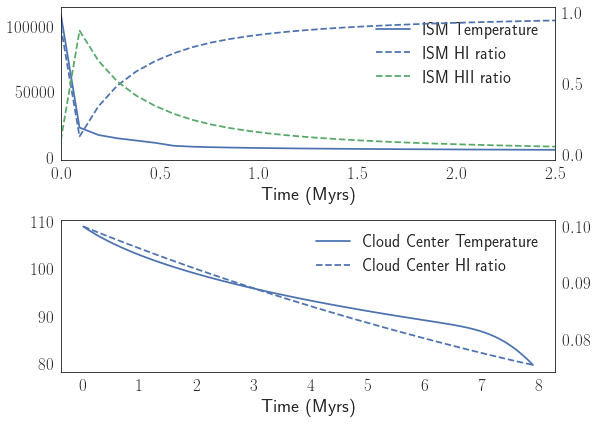
\includegraphics[width=1\linewidth]{DataImages/H2CoolingTMPcenterISM}
	\caption{}
	\label{fig:h2coolingtmpcenterism}
\end{figure}

%
%	Οι παρατηρήσεις των μοριακών νεφών μας δίνουν θερμοκρασίες της τάξεως των $\SI{30}{K}$. Η ασυμφωνία με την προσομοίωση εξηγείται καθώς 
	\begin{figure}[h]
		\centering
		\includegraphics[width=1\linewidth]{DataImages/Η2cooling-function}
		\caption{}
		\label{fig:h2cooling-function}
	\end{figure}
	
% Και
%
%Αν χρησιμοποιούσαμε χαμηλότερη θερμοκρασία (για παράδειγμα τους \SI{30}{K}) τότε το αέριο θα διατηρούταν σε αυτή τη θερμοκρασία. Επειδή όμως θέλαμε να μελετήσουμε τη ψύξη στο νέφος αποφύγαμε να "επιβάλλουμε" τη δική μας αποδεκτή θερμοκρασία.

%\begin{figure}[h]
%	\centering
%	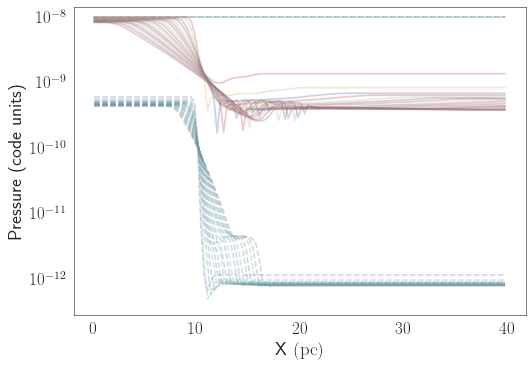
\includegraphics[width=1\linewidth]{DataImages/diffH2CoolSNCoolPRSprofile.png}
%	\caption{Σύγκριση του προφίλ της πίεσης για το}
%	\label{fig:diffh2coolsncoolprsprofile}
%\end{figure}
 Συμπεραίνουμε λοιπόν ότι παρότι το H2Cool αποδίδει πολύ καλύτερα από το SNEq σαν module που εκτελεί ταυτόχρονα και χημικές διεργασίες, η συμπεριφορά του στις πολύ χαμηλές θερμοκρασίες είναι ανεπαρκής λόγω έλλειψης των γραμμών εκπομπής των μορίων \ce{CO}, \ce{OH} και \ce{H2O}.

 Έτσι στη συνέχεια θα χρησιμοποιήσουμε σαν βέλτιστη επιλογή το Tabulated Cooling Module.

	\newpage
	
	\section{Βαρύτητα}
	Είναι προφανές ότι έναν από τους ισχυρότερους ρόλους στην αστροφυσική (αν όχι το μεγαλύτερο) τον παίζει η βαρύτητα. 
	
	\subsection{Self Gravity}
	\label{par:SolidSphereSelfGravit}
	Επειδή ο PLUTO δεν μπορεί να χειριστεί την ιδιοβαρύτητα θα προσπαθήσουμε να τη προσεγγίσουμε τοποθετώντας ένα βαρυτικό δυναμικό ομογενούς σφαίρας στο εσωτερικό του νέφους και ένα δυναμικό σημειακής μάζας στο εξωτερικό του νέφους. Δηλαδή:
	\begin{equation}
		\vec{g}(x,y) = 
		\begin{cases}
			\frac{GM}{R^3}(x \hat{x}+ y \hat{y}) &\texttt{if } r<R \\
			\frac{GM}{r^3}(x \hat{x}+ y \hat{y}) &\texttt{if } r>R
		\end{cases}
	\end{equation}
	
	όπου $r=\sqrt{x^2+y^2}$
	
	\subsubsection{Βαρυτική Σταθερά}
	Για να χρησιμοποιήσουμε τη δύναμη της βαρύτητας θα πρέπει να υπολογίσουμε τη σταθερά $G$ σε μονάδες κώδικα, όπως βλέπουμε και από το πίνακα~\ref{tab:cd}. Άρα 
	\begin{equation}
		G=G_\texttt{cgs} \si{cm^3.g^{-1}.s^{-2}} = G_\texttt{cgs} \frac{\SI{1.67e-24}{g.cm^{-3}}}{\rho_0}\frac{10^{18}\si{s^2}}{t^2_0}
	\end{equation}
	Αντικαθιστώντας $G_\texttt{cgs}=\SI{6.674e-8}{}$ βρίσκουμε
	\begin{equation}
		\boxed{G=\SI{1.114e-13}{G_0}}
	\end{equation}
	όπου $G_0=(\rho_0 t_0)^{-1}$ η σταθερά της βαρύτητας σε μονάδες κώδικα.
	
%	\begin{marginfigure}
%		\includegraphics[width=1.0\linewidth]{astro/Diplomatiki/logDensityG}
%		\caption{Density Simulation (Logarithmic Scale) over four different times in one $t_\texttt{ff}$.}
%		\label{fig:logdensityg}
%	\end{marginfigure}
	
	\subsubsection{Χρόνος Ελεύθερης Πτώσης}
	Ο χρόνος ελεύθερης πτώσης (free-fall time) είναι η χρονική κλίμακα που χρειάζεται ένα σώμα να καταρρεύσει κάτω από το ίδιο το βάρος του, αν δεν υπεισέρχονται άλλες δυνάμεις που να αντισταθμίσουν ή να επιταχύνουν τη διαδικασία. Έτσι παίζει ένα πολύ σημαντικό ρόλο στις χρονικές κλίμακες πολλών αστροφυσικών διεργασιών.
	
	Στη περίπτωση του δικού μας νέφους ο χρόνος ελεύθερης πτώσης υπολογίζεται:
	\begin{equation}
		t_\texttt{ff}=\sqrt{\frac{3\pi}{32G\rho}} = \SI{51404}{t_0} = \SI{1.6}{Myrs}
	\end{equation}
	
	\subsection{Σφαιρικό νέφος μέσα σε βαρυτικό δυναμικό χωρίς Ψύξη}
	
	Για να εξετάσουμε την επίδραση της βαρύτητας αρχικά θα εκτελέσουμε την προσομοίωση που έχουμε κάνει και προηγουμένως, αρχικά σε ένα νέφος που δεν εμπεριέχει διαδικασία ψύξης.
	
\begin{figure}[h]
	\centering
	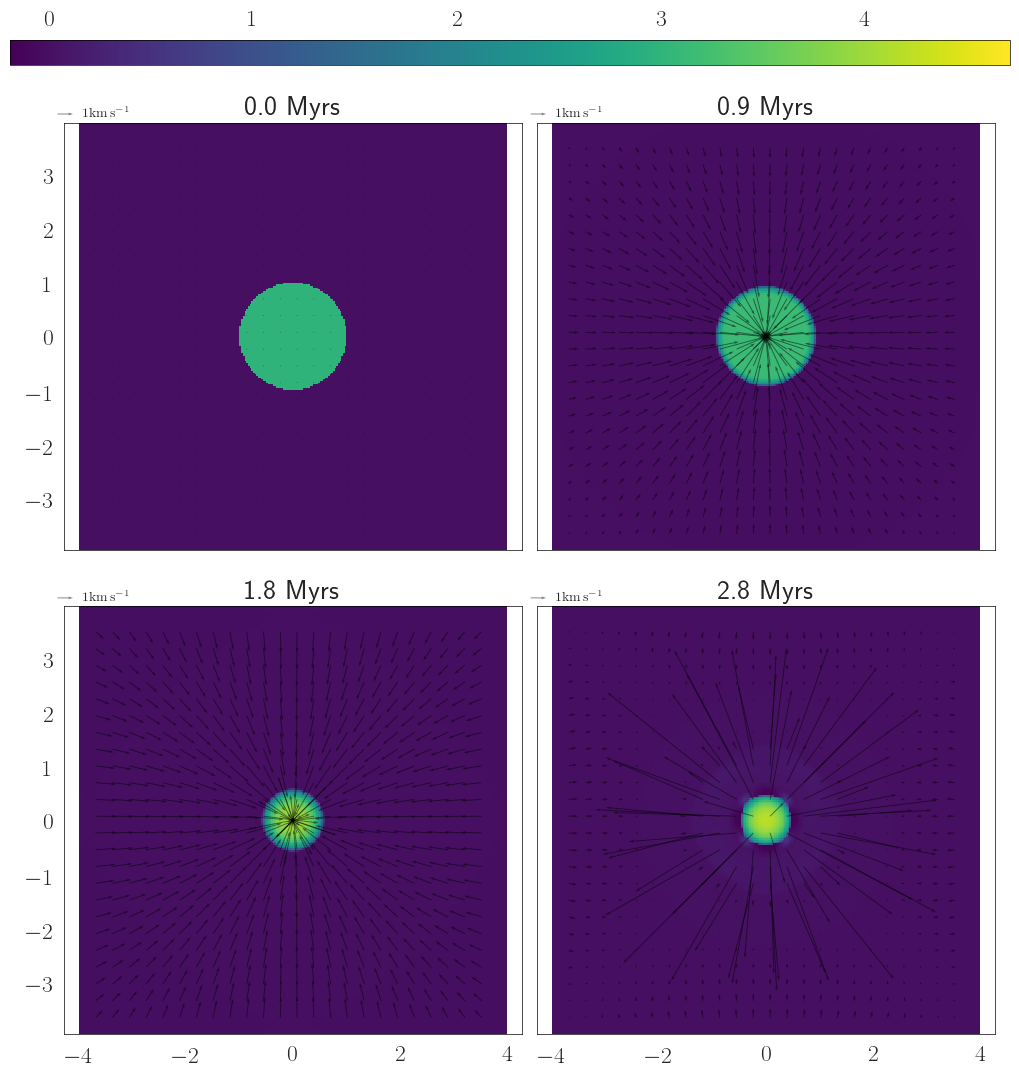
\includegraphics[width=1\linewidth]{DataImages/NoCoolGRquad}
	\caption{Ο χάρτης της πυκνότητας (λογαριθμική κλίμακα) σε 4 διαδοχικά στιγμιότυπα έως και λίγο αργότερα από το χρόνο κατάρρευσης. Η εσωτερική πίεση του νέφους το διογκώνει έως η βαρύτητα αργότερα να το επαναφέρει.}
	\label{fig:nocoolgrquad}
\end{figure}

\begin{marginfigure}
	\centering
	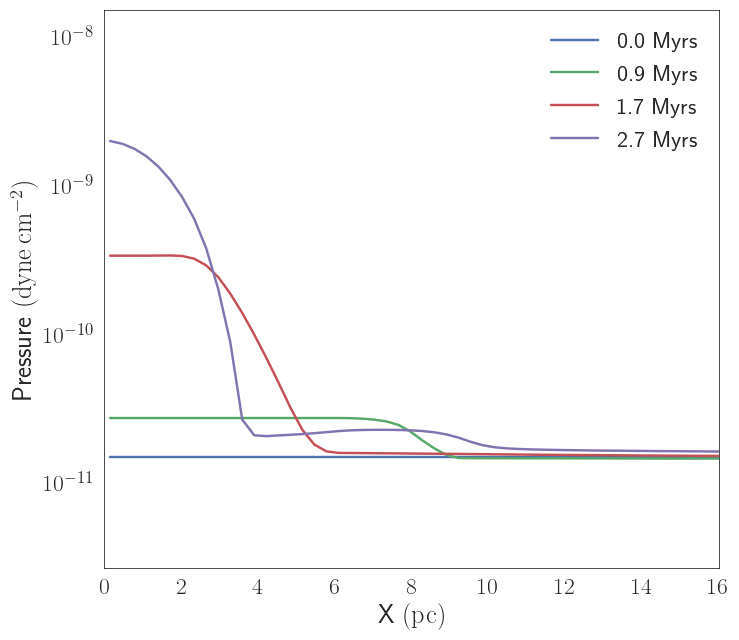
\includegraphics[width=1\linewidth]{DataImages/NoCoolGPRSprofile.png}
	\caption{Το προφίλ τη πίεσης σε 4 διαδοχικά στιγμιότυπα μέχρι και λίγο αργότερα από το χρόνο κατάρρευσης.}
	\label{fig:nocoolgprsprofile}
\end{marginfigure}

Το αποτέλεσμα όπως φαίνεται από το σχήμα~\ref{fig:nocoolgrhoprofile} δείχνουν ένα χρόνο κατάρρευσης κοντά στα $\SI{2}{Myrs}$ καθώς στη συνέχεια το νέφος αναπηδά λόγω της θερμικής πίεσης (σχήμα~\ref{fig:nocoolgprsprofile}) και επιταχύνεται προς τα έξω.
Το αποτέλεσμα είναι πολύ κοντά στην τιμή του χρόνου ελεύθερης πτώσης καθώς η πίεση δεν ήταν αρκετή για να επιβραδύνει νωρίτερα την κατάρρευση και επίσης η ακρίβεια των προσομοιώσεων δεν είναι αρκετή για να διαχειριστεί απόλυτα σωστά το φαινόμενο της βαρυτικής κατάρρευσης. Ένα pixel αντιστοιχεί σε $\SI{0.3125}{parsec}\simeq \SI{1}{ly}$ μέγεθος πολύ μεγαλύτερο από ένα πρωτοαστέρα που θεωρούμε ότι είναι το αναμενόμενο αποτέλεσμα της βαρυτικής κατάρρευσης.

\subsection{Σφαιρικό νέφος σε βαρυτικό δυναμικό με Radiation Cooling}

Στη συνέχεια θα επαναλάβουμε τη προσομοίωση της βαρυτικής κατάρρευσης μαζί με τη ψύξη του αερίου.
% Επειδή μας ενδιαφέρει να μελετήσουμε και τη μοριακή σύσταση (για το \ce{H2} προς το παρόν) θα χρησιμοποιήσουμε το module H2COOL το οποίο κρίνουμε ικανοποιητικό για τις χαμηλές τουλάχιστον θερμοκρασίες.
Επειδή κρίναμε ότι τελικά το Tabulated Cooling αποδίδει τα καλύτερα δυνατά αποτελέσματα για τις χαμηλές θερμοκρασίες θα το χρησιμοποιήσουμε για τη προσομοίωση της ψύξης του νέφους.
\begin{figure}[h]
	\centering
	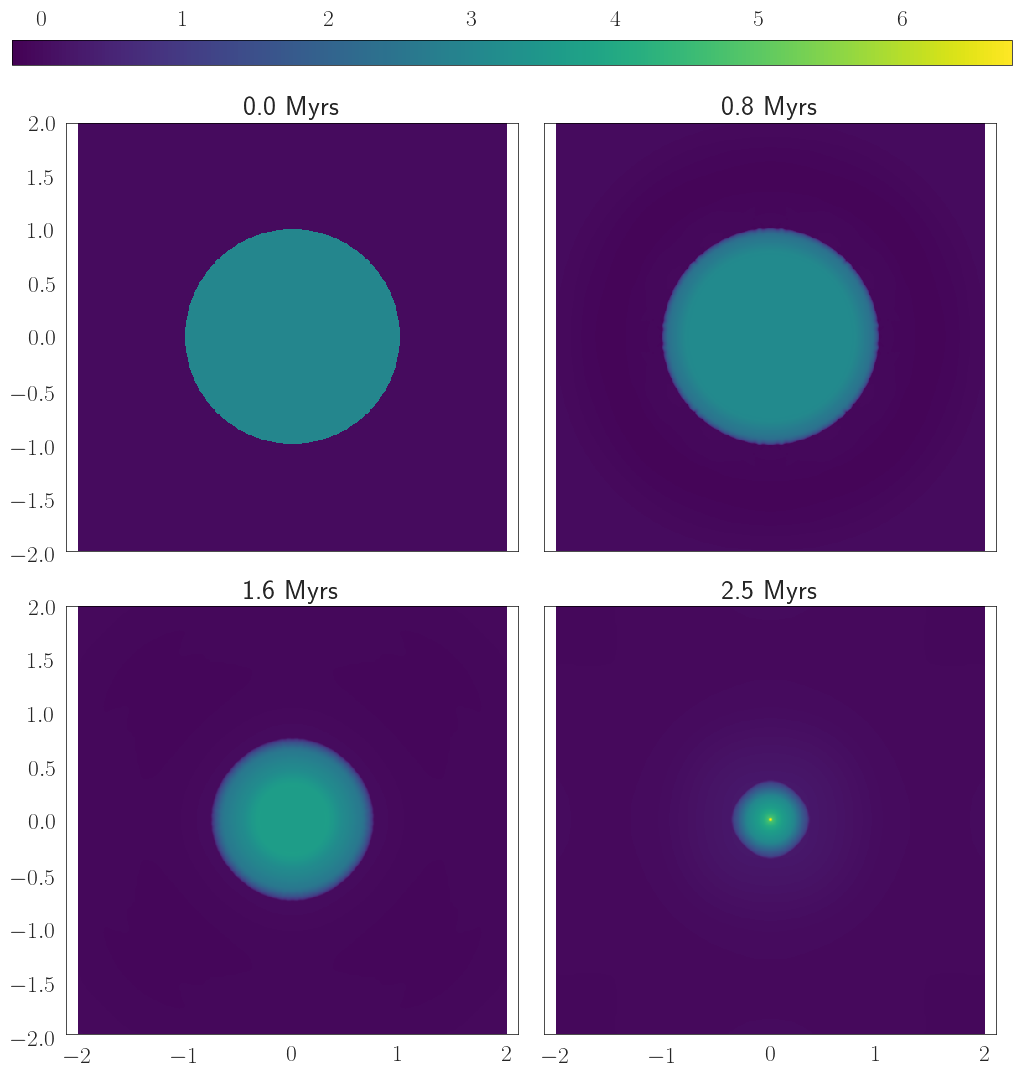
\includegraphics[width=1\linewidth]{DataImages/H2CoolGRquad}
	\caption{Ο χάρτης της πυκνότητας (λογαριθμική κλίμακα) σε 4 διαδοχικά στιγμιότυπα μέχρι το χρόνο κατάρρευσης. }
	\label{fig:h2coolgrquad}
\end{figure}

\begin{marginfigure}
	\centering
	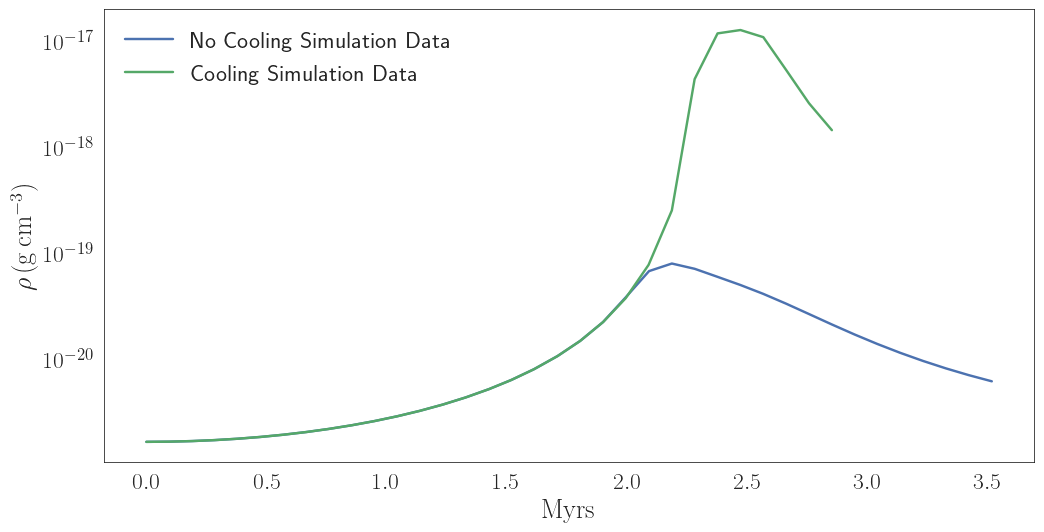
\includegraphics[width=1\linewidth]{DataImages/GRcenterTimeRHO}
	\caption{Πυκνότητα στο κέντρο του νέφους σε σχέση με το χρόνο για τις δύο προσομοιώσεις.}
	\label{fig:grcentertimerho}
\end{marginfigure}


Για τη συγκεκριμένη προσομοίωση χρησιμοποιήσαμε μεγαλύτερη ανάλυση (512X512 pixel) και χρονική ανάλυση στα \SI{95}{kyrs}. Θεωρούμε σαν χρόνο κατάρρευσης το χρόνο εκείνο όπου η κεντρική περιοχή αποκτά τη μέγιστη πυκνότητα. Έτσι υπολογίζουμε 
\begin{equation}
t_\mathtt{col}=\SI{2.47\pm 0.05}{Myrs}
\end{equation}
με τη μέγιστη πυκνότητα να έχει τιμή
\begin{equation}
\rho _\mathtt{max}=\SI{1.29e-17}{g.cm^{-3}}
\end{equation}


	
	\subsubsection{Σφαίρα Bonnor-Ebert}
	Αν θεωρήσουμε ένα οπτικά διαφανές, σφαιρικό μοριακό νέφος το οποίο βρίσκεται σε ισορροπία πιέσεων και η θερμοκρασία του διατηρείτε σταθερή (δηλαδή το πλεόνασμα ενέργειας από τη βαρυτική κατάρρευση εξισορροπείτε από την ψύξη μέσω της εκπομπής ακτινοβολίας) τότε θα έχουμε:

	\begin{align}
	\frac{GM_r}{r^2} +\frac{1}{\rho}\frac{dP}{dr}=0  &\qquad \text{Εξίσωση Κίνησης}\\
	\frac{dM_r}{dr} = 4 \pi r^2 \rho &\qquad \text{Εξίσωση Διατήρησης της Μάζας}\\
	P = c_s ^2 \rho &\qquad \text{Καταστατική Εξίσωση}
	\end{align}
	
	Συνδυάζοντας και τις τρεις έχουμε την εξίσωση Emden:
	\begin{equation}
	\frac{1}{r^2}\frac{d}{dr} \left( r^2 c_s ^2 \frac{d \ln \rho}{dr}\right)  = -4 \pi G \rho
	\end{equation}
	
	Θα επικεντρωθούμε στην απλούστερη λύση αυτής της εξίσωσης, όπου η κεντρική πυκνότητα είναι άπειρη (λύση SIS - Singular Isothermal Sphere):
	\begin{equation}
	\label{eq:B-E_density}
	\rho _\mathtt{BE}(r) =\frac{c_s ^2}{2 \pi G} \frac{1}{r^2}
	\end{equation}

 Ρεαλιστικότερες λύσεις - χωρίς ασυνέχειες στο κέντρο της σφαίρας - προσεγγίζονται ικανοποιητικά με τη παραπάνω εξίσωση μέχρι μια κρίσιμη απόσταση $r_c=\frac{c_s}{\sqrt{4\pi G \rho _c}}$ όπου $\rho _c$ η πυκνότητα στο κέντρο $(r=0)$.  Η θεωρητική αυτή κατανομή πυκνοτήτων ονομάζεται σφαίρα Bonnor - Ebert.
 
  \begin{figure}[h]
 	\centering
 	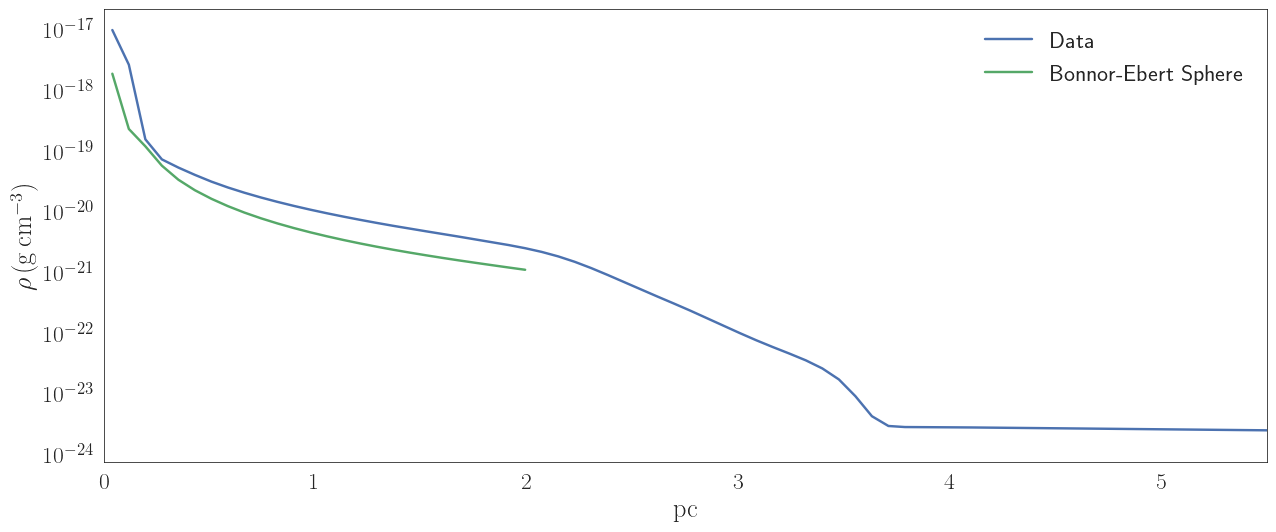
\includegraphics[width=1\linewidth]{DataImages/H2CoolGRHOprofile-BE}
 	\caption{Σύγκριση των κατανομών πυκνοτήτων για τις δύο προσομοιώσεις σε σχέση με το θεωρητικό μοντέλο της σφαίρας Bonnor - Ebert. Το χρονικό στιγμιότυπο αντιστοιχεί στο χρόνο κατάρρευσης της κάθε προσομοίωσης. }
 	\label{fig:h2coolgrhoprofile-be}
 \end{figure}
 
 
 Η κρίσιμη απόσταση για μια κεντρική πυκνότητα της τάξης των \SI{1e-19}{g.cm^{-3}} βρίσκεται στα περίπου \SI{0.1}{pc}. Για τη προσομοίωση μας η απόσταση αυτή αντιστοιχεί στα \SI{1.2}{pixel}, επομένως για να συγκρίνουμε επικεντρωνόμαστε στη SIS λύση. Στο γράφημα \ref{fig:h2coolgrhoprofile-be} δείχνουμε τη κατανομή της σφαίρας Bonnor - Ebert μαζί με τις προσομοιώσεις με ή χωρίς ψύξη στον αντίστοιχο χαρακτηριστικό χρόνο κατάρρευσης.  
 

 Παρατηρούμε ότι η προσομοίωση συμφωνεί με το θεωρητικό μοντέλο της σφαίρας Bonnor - Ebert και κατ' επέκταση με παρατηρησιακά δεδομένα \todo{Citation needed}.  



\begin{marginfigure}
	\centering
	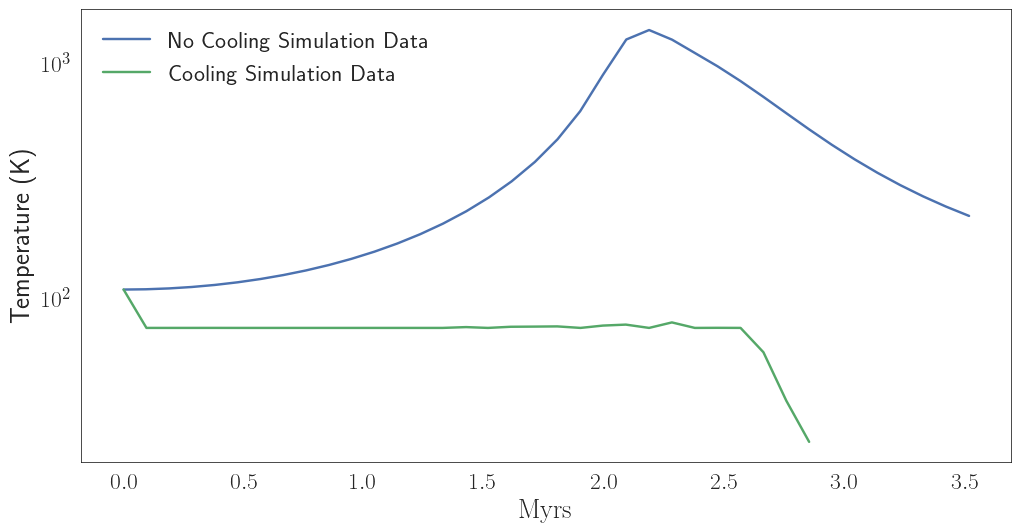
\includegraphics[width=1\linewidth]{DataImages/GRcenterTimeTemp}
	\caption{Θερμοκρασία στο κέντρο του νέφους σε σχέση με το χρόνο της προσομοίωσης. Παρατηρούμε ότι η προσομοίωση με ενεργοποιημένο το H2COOL διατηρεί τη θερμοκρασία σχεδόν σταθερή μέχρι τη τελική κατάρρευση του νέφους.}
	\label{fig:grcentertimetemp}
\end{marginfigure}

Από το γράφημα \ref{fig:grcentertimetemp} βλέπουμε τη διαφορά στις θερμοκρασίες του νέφους για τις δύο προσομοιώσεις. Όταν έχουμε ψύξη το πλεόνασμα ενέργειας ακτινοβολείται διατηρώντας τη θερμοκρασία σε καλή προσέγγιση σταθερή μέχρι τη τελική κατάρρευση με αποτέλεσμα να έχουμε τη συμφωνία με τη σφαίρα Bonnor - Ebert. 


\subsubsection{Τεχνητή κατανομή πυκνότητας}
Όπως αναφέραμε και προηγουμένως ο PLUTO δεν μπορεί να ολοκληρώσει την εξίσωση Gauss άρα δεν μπορούμε να μελετήσουμε τα αποτελέσματα της ιδιοβαρύτητας όπως για παράδειγμα το φαινόμενο της ιεραρχικής κατακρήμνισης και τη δημιουργία των πυκνών μοριακών πυρήνων που θα μας δώσουν αστέρες (στο παραπάνω παράδειγμα παρατηρούμε τη δημιουργία μόνο ενός τέτοιου πυρήνα). 

Η ενασχόληση μας όμως με τη προσθήκης του "τεχνητού" βαρυτικού δυναμικού στις προσομοιώσεις μας απέδωσε μια αποδεκτή κατανομή πυκνότητας για ένα σφαιρικό νέφος. Έτσι για φαινόμενα με χαρακτηριστική χρονική κλίμακα μικρότερη του χρόνου ελεύθερης πτώσης $t_\mathtt{ff}$ μπορούμε να χρησιμοποιούμε μια κατανομή σαν αυτή που παρατηρήσαμε στη προηγούμενη προσομοίωση αντί για μια μη ρεαλιστική σταθερή (και πολύ μεγάλης συνολικής μάζας) κατανομή όπως κάναμε στο προηγούμενο κεφάλαιο.

Για να μην αποφύγουμε αριθμητικές αστάθειες στο κέντρο του νέφους αλλά και για πιο ρεαλιστική κατανομή της πυκνότητας θα γενικεύσουμε τη σχέση της κατανομής της πυκνότητα Bonnor - Ebert. εισάγοντας σαν παραμέτρους τη πυκνότητα στο κέντρο του νέφους $\rho _c$, μια κρίσιμη ακτίνα απ' όπου η πυκνότητα σταθεροποιείται $r_c$ και ένα νόμο δύναμης για το τρόπο με τον οποίο μειώνεται. 


\begin{marginfigure}
	\centering
	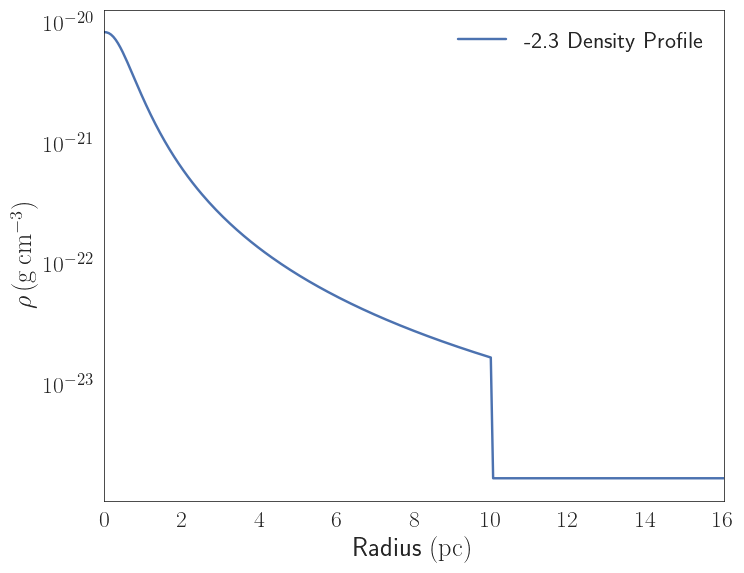
\includegraphics[width=1\linewidth]{DataImages/SimRHOProfile}
	\caption{Κατανομή της πυκνότητας συναρτήσει της ακτίνας στο μοντέλο τύπου Plummer του μοριακού νέφους. }
	\label{fig:simrhoprofile}
\end{marginfigure}

\begin{marginfigure}
	\centering
	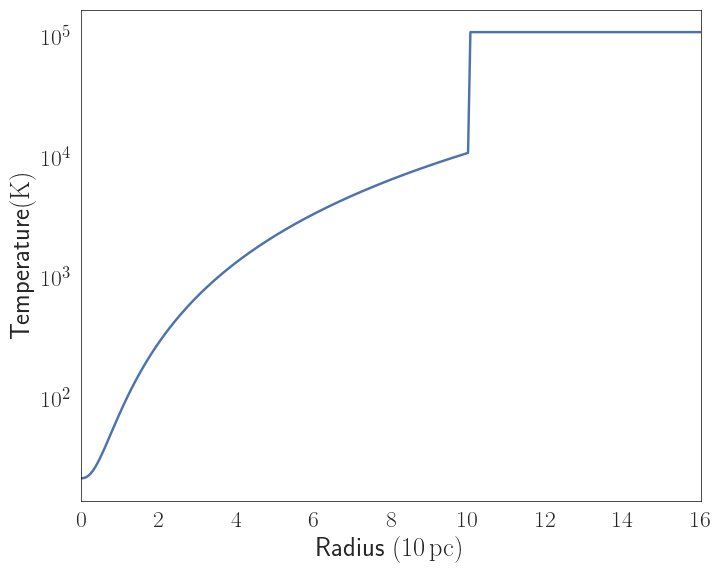
\includegraphics[width=1\linewidth]{DataImages/SimTMPProfile}
	\caption{Κατανομή θερμοκρασίας συναρτήσει της ακτίνας δεδομένης της αρχικής πίεσης.}
	\label{fig:simtmpprofile}
\end{marginfigure}


Έτσι θα χρησιμοποιήσουμε μια κατανομή της μορφής Plummer:
\begin{equation}
\rho (r)=\frac{A}{B+r^a}
\end{equation}
όπου $A=\rho _c r_c^a$, $B=r_c^a$ με $a$ το νόμο δύναμης. 


Από τη κατανομή που μας δίνει η προσομοίωση υπολογίζουμε μέσω της μεθόδου των ελαχίστων τετραγώνων τη τιμή για το νόμο δύναμης
\begin{equation}
a=\num{2.3\pm 0.14}
\end{equation}

Όπως αναφέραμε προηγουμένως η προσομοίωση μας δεν μπορεί να περιγράψει απόλυτα ρεαλιστικά ένα μοριακό νέφος. Γι αυτό το λόγο δεν προσπαθούμε να να προσαρμόσουμε μια -πολύπλοκη- καμπύλη πυκνοτήτων πάνω στα αποτελέσματα μας, παρά να μελετήσουμε μια γενικότερη συμπεριφορά και να κρίνουμε αν η ψύξη λειτουργεί σε ικανοποιητικό βαθμό. 


Έτσι παρότι κρατήσαμε τη τιμή του νόμου δύναμης, η εκτίμηση των υπολοίπων παραμέτρων θα γίνει περισσότερο "εμπειρικά" με βάση τα όσα γνωρίζουμε από πραγματικά παρατηρούμενα μοριακά νέφη. Θεωρώντας μια ακτίνα ενός μέσου μοριακού νέφους στα \SI{10}{pc} και μια συνολική μάζα τάξης \SI{1e3}{M_\odot} ταυτόχρονα με τη συνθήκη η πυκνότητα στο άκρο του νέφους να μην έχει μεγάλη διαφορά πολύ από αυτή του μεσοαστρικού αερίου κάναμε μια εκτίμηση των παραμέτρων
\begin{align}
A=10 && B=0.002
\end{align}

Έτσι υπολογίζουμε
\begin{align}
\rho _c = \frac{A}{B}= \SI{5000}{cm^{-3}} && r_c = B^{1/a} = \SI{0.67}{pc}
\end{align}
 
Η τελική κατανομή, όπως και η κατανομή της θερμοκρασίας στο νέφος με δεδομενή την πίεση φαίνονται στα διαγράμματα (\ref{fig:simrhoprofile},\ref{fig:simtmpprofile})

Κάπου εδώ ολοκληρώνεται η διαδικασία του "χτισίματος" ενός μοριακού νέφους έτσι ώστε να χρησιμοποιηθεί σε μεγάλης κλίμακας προσομοίωση. Δοκιμάζοντας βήμα βήμα τις δυνατότητες του PLUTO καταφέραμε τελικά να δημιουργήσουμε μια όσο το δυνατόν ρεαλιστική απεικόνιση ενός μοριακού νέφους.  



























